\part{Développement de l'interface}
	
	\chapter{L’utilisation d’images IIIF}
	Ce chapitre a pour objet le protocole \acrshort{iiif} (\acrlong{iiif}. Il s'agit de présenter d'abord la communauté \acrshort{iiif} et certaines institutions qui en font partie avant de se consacrer à la présentation d'outils qui s'appuient sur des images \acrshort{iiif} et qui sont utiles à la conception d'une exposition virtuelle. 
	
	\section{Communauté IIIF}
	\subsection{Généralités}
	\acrshort{iiif} \footnote{Les informations générales présentées ici sont issues de la documentation relative à ce protocole et accessible sur le \href{https://iiif.io/get-started/how-iiif-works/}{site web du \textit{framework}}.} peut désigner deux choses : un consortium dont font partie de nombreux acteurs des humanités numériques et un protocole \textit{open source}. On se focalisera ici sur les images mais ce protocole existe aussi pour des fichiers audio. \acrshort{iiif} est un modèle \textit{open source} qui donne accès à grande échelle, en ligne, à des objets numériques. Outre la haute qualité de ces objets, l'une des forces des objets \acrshort{iiif} est de permettre à ceux qui les visualisent d'interagir avec les images ainsi accessibles : il est notamment possible de zoomer à différentes échelles tout en conservant l'excellente qualité de l'image visionnée ou bien de les annoter. La comparaison d'images est également possible et intuitive y compris pour des images originellement conservées dans des institutions différentes qui deviennent ainsi manipulables de façon homogène. C'est là l'un de points forts de ce protocole : son interopérabilité. C'est quelque chose qui faisait défaut aux institutions patrimoniales mais qui s'est révélé nécessaire à l'heure où les échanges numériques se font de plus en plus fréquents. Un autre atout est de pouvoir réutiliser des images hébergées par un autre projet. \acrshort{iiif} offre aussi un cadre pour la description des ressources en ligne avec des métadonnées standardisées. 
	
	On note deux composantes principales du protocole \acrshort{iiif} : une \acrshort{api} image et une \acrshort{api} présentation. L'\acrshort{api} image est la norme qui permet la communication entre le serveur et le client : le premier stocke les images tandis que le second les affiche dans un navigateur web. L'image peut ou non être entière, il peut s'agir d'une portion zoomée, d'une version inclinée différemment ou encore en noir et blanc, ce sont les paramètres de l'\acrshort{url} qui déterminent cela. 

    L'\acrshort{api} présentation correspond quant à elle aux métadonnées associées à la ressources et à sa structure grâce au \textit{manifest}. C'est un fichier \acrshort{json} qui contient des informations relatives au stockage des images, à leur affichage, à l'ordre des pages mais également des métadonnées élémentaires comme le titre, la description et les droits de l'image. L'\acrshort{api} présentation comporte aussi un autre fichier \acrshort{json} nommé info qui, lui, indique quelles sont les manipulations de l'image autorisées par le serveur image. 
    
    En plus de proposer un cadre et des recommandations, la communauté \acrshort{iiif} est aussi à l'origine de la création de guides et tutoriels pour créer des contenus \acrshort{iiif} ou pour réutiliser ceux qui existent déjà. Parmi ces outils, il faut évoquer la semaine de \textit{workshops} animée par Glen Robson \footnote{Ces \textit{workshops} ont lieu plusieurs fois par an et sont accessibles gratuitement \href{https://training.iiif.io/iiif-online-workshop/}{en ligne}.} pour présenter ce qu'il est essentiel de connaître et de comprendre pour se lancer dans l'utilisation de ressources \acrshort{iiif}.

	\subsection{IIIF dans les institutions patrimoniales}
	Ainsi, nombreuses sont les institutions qui prennent part à cette communauté. C'est par exemple le cas de bibliothèques nationales comme la \acrlong{bnf}, l'\acrlong{onb}, la \acrlong{bl} ou encore la \acrlong{lc} mais aussi de musées ou d'universités. Pour une institution conservant des manuscrits ou des chercheurs travaillant sur ce même type de source, un intérêt d'utiliser des images \acrshort{iiif} réside dans la possibilité offerte par ce \textit{framework} de reconstituer des manuscrits. Il est possible de réunir en une collection des pages désormais séparées dans plusieurs institutions de conservation afin de recréer numériquement le manuscrit de départ. 
	
	Tous les manuscrits choisis pour l'exposition \acrshort{alfa} ne sont pas accessibles en \acrshort{iiif}. Ceux qui le sont sont conservés à la \acrlong{bnf} et à l'\acrlong{ub} d'Erfurt. Dans ces cas là, la récupération des \textit{manifests} est simple et se fait directement via le visualiseur Mirador où l'on peut obtenir l'\acrshort{url} du \textit{manifest}. Autre bibliothèque proposant un accès à ses documents au format \acrshort{iiif}, la \acrlong{bav} présente pourtant des difficultés pour l'utilisation de ces ressources à des fins d'exposition en ligne. En effet, le manuscrit Pal. lat. 1375 est consultable sur le site Digivatlib, bibliothèque en ligne de la \acrlong{bav}, grâce au visualiseur Mirador. De même, sur le \textit{survey} réalisé pour le projet \acrshort{alfa}, la visualisation \acrshort{iiif} fonctionne elle aussi. Néanmoins, lorsqu'on reporte l'\acrshort{url} dans l'outil Exhibit, choisi pour réaliser l'exposition, la visualisation ne fonctionne pas. Cela peut venir de l'\acrshort{api} Authentification. En effet, cela permet de bloquer certaines réutilisations et c'est ce qui semble se passer ici. Ainsi, si l'accès est bloqué, pour un contenu intégré, seule une icône d'image apparaît sans que l'image ne se charge. Cela peut être considéré comme une participation particulière au consortium \acrshort{iiif} car cela ne correspond pas aux principes de réutilisation et d'\textit{open source}. De plus, l'intégralité des numérisations de la \acrlong{bav} sont revêtues d'un \textit{copyright}, ce qui, là encore, semble aller à l'encontre de l'\textit{open source}. Aussi pour ce manuscrit ainsi que pour ceux dont les numérisations existent mais ne sont pas au format \acrshort{iiif}, il a fallu créer des \textit{manifests.}
	
	\subsection{Créer un \textit{manifest}}
	La création d'un \textit{manifest} peut se faire en suivant les indications du \textit{workshop} précédemment mentionné. Cela peut être fait en quelques étapes assez simple à commencer par le téléchargement de la numérisation du manuscrit pour lequel on veut créer un \textit{manifest}. Il faut ensuite se rendre sur \href{https://workbench.gdmrdigital.com/}{IIIF Workbench} et se connecter avec son compte Github, ou en créer un le cas échéant. À partir de là, il est possible de créer un nouveau projet ou d'en sélectionner un déjà existant que l'on souhaiterait retravailler. L'étape suivante est un chargement des images, une fois une image chargée, on peut obtenir le lien du fichier \texttt{info.json}.  
	
	Une fois ce lien obtenu, il faut se rendre sur le \href{https://digital.bodleian.ox.ac.uk/manifest-editor/#/?_k=xqu304}{Bodleian Manifest Editor} et choisir \textit{New manifest} et attribuer un nom au \textit{manifest} dans les paramètres liés aux métadonnées du \textit{manifest}. Un canva vide a normalement été créé et les métadonnées liées à celui-ci peuvent à leur tour être complétées. Après avoir cliqué sur le bouton \textit{+ Add Image to Canvas}, une fenêtre \textit{popup} s'ouvre et elle permet d'ajouté le fichier \acrshort{json} précédemment créé en utilisant \textit{From \texttt{info.json} URI} puis en cliquant sur \textit{Submit URI}. Un titre doit ensuite être ajouté au canva. Il faut procéder de la sorte pour toutes les images qui doivent être ajoutées au \textit{manifest}. Quand c'est chose faite, un simple clic sur \textit{Save Manifest} permet d'enregistrer le \textit{manifest}. Il est également posisble d'éditer un fichier \texttt{manifest.json} déjà existant en procédant de la même manière.
	
	Pour terminer la création, il faut retourner sur \href{https://workbench.gdmrdigital.com/}{IIIF Workbench} et cliquer sur le bouton \textit{Manifests} dans la barre de navigation. Il est alors possible de charger le \textit{manifest} qui vient d'être sauvegardé. Enfin, le lien du fichier \texttt{manifest.json} peut enfin être obtenu et être ensuite utilisé dans différents outils. 
	
	Pour cette exposition, j'ai donc pu créer des \textit{manifests} pour quatre manuscrits : ceux conservés à la \acrlong{bav}, à l'\acrlong{onb}, à la \acrlong{bne} et à la \acrlong{rbme}. Cela m'a permis à la fin de mon stage de créer les \textit{exhibits} de ces manuscrits et d'ajouter les \textit{attention points} dans les parcours concernés \footnote{Des précisions sur la création des \textit{exhibits} sont apportées à la fin de ce chapitre.}.
	

    \section{Outils IIIF pour développer une exposition en ligne}
    Les outils \acrshort{iiif} sont nombreux et permettent aux utilisateurs d'avoir accès à différentes fonctionnalités comme annoter ou recadrer une image sur une partie précise. Certains outils ont aussi été développés pour aider à la création de contenu d'exposition virtuelle, ce sont ceux qui vont donc nous intéresser. 
    
	\subsection{Outils envisagés}
	\subsubsection{Storiiies Editor}
	Parmi ces outils, il faut commencer par présenter Storiiies Editor qui est décrit comme une plateforme de \textit{storytelling} en ligne permettant de créer des visites guidées à l'aide d'annotations relatives à un unique \textit{manifest}. C'est cet outil qui avait été envisagé dans un premier temps pour préparer le contenu de l'exposition par l'équipe du projet \acrshort{alfa}. En effet, les \textit{attention points}, texte et image, avaient été entrés sur cette plateforme pour un certain nombre de manuscrits. 
	
	\begin{figure}[h]
	\caption{Interface d'édition de Storiiies}
	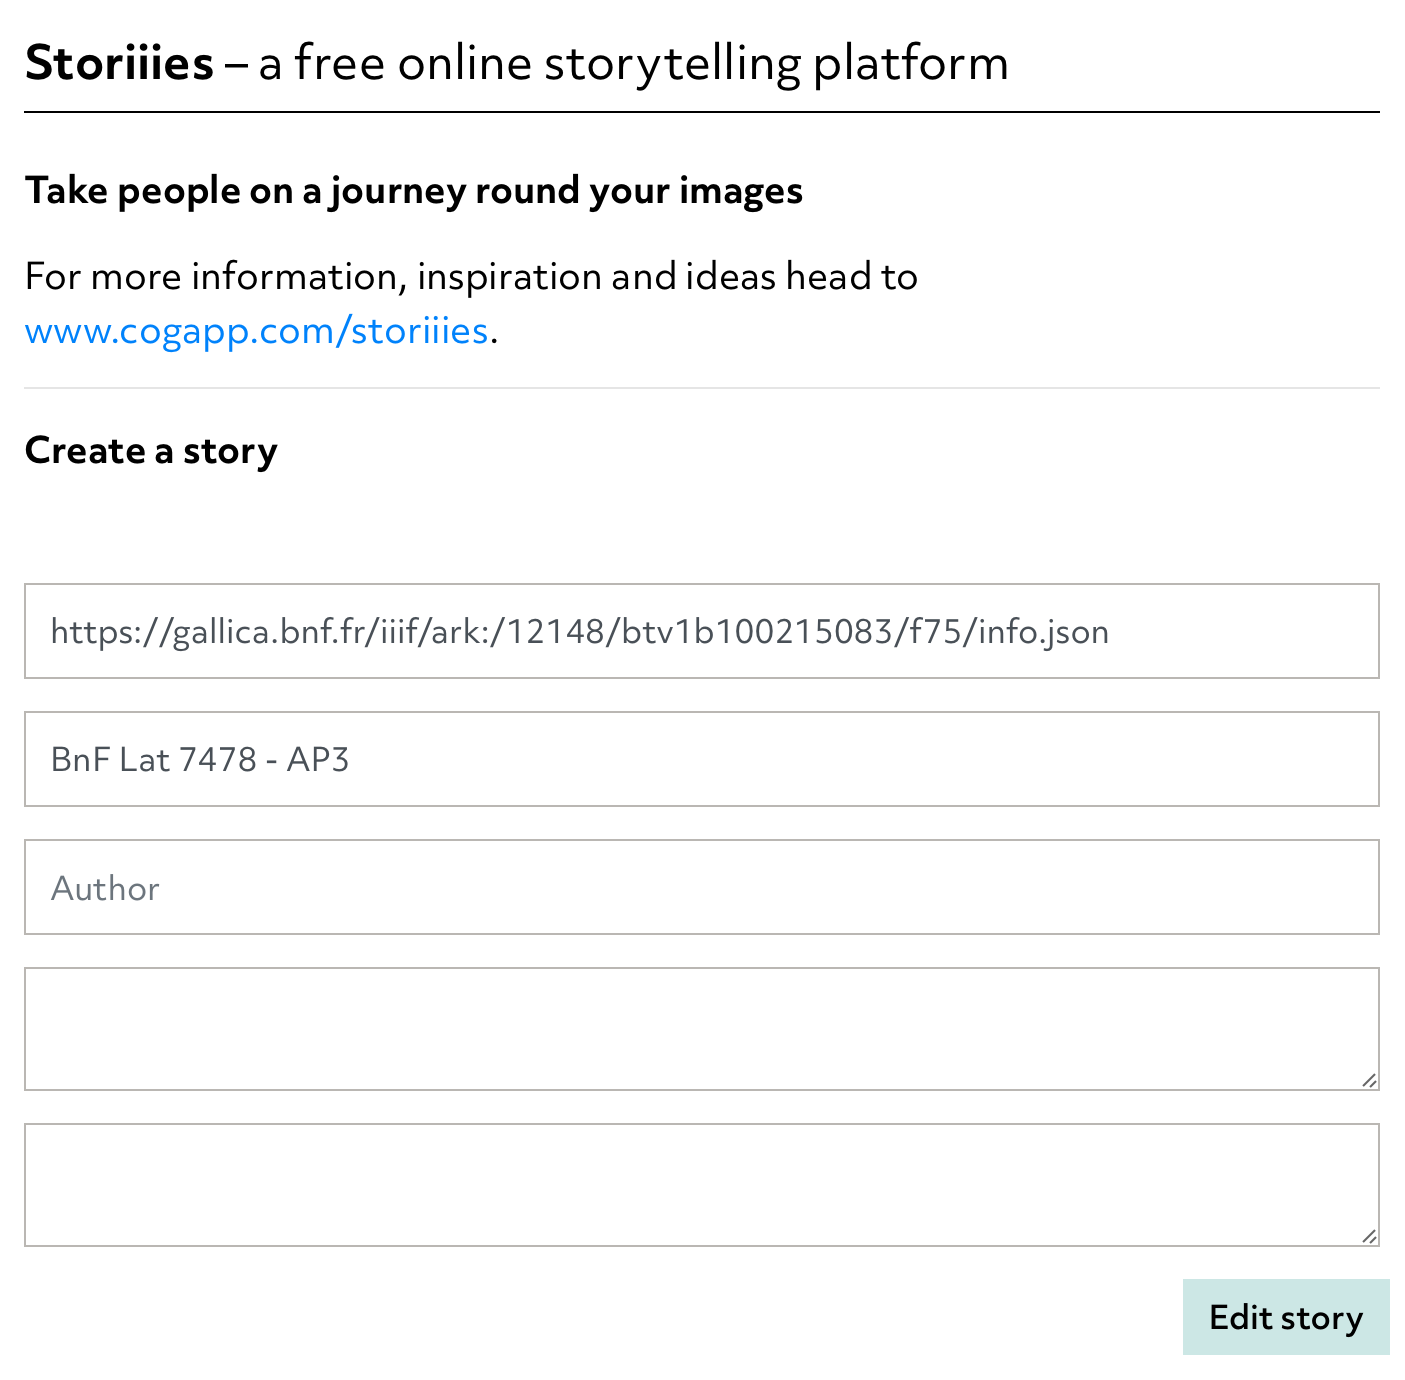
\includegraphics[scale=0.4, angle=0]{images/partie3/storiiies/storiiies-editor.png}
    \centering
    \end{figure}
	
	L'interface d'édition est minimale, ce qui rend sa prise en main très simple. Il suffit d'ajouter le lien du fichier \texttt{manifest.json}, récupéré sur le site d'une institution ou créé selon la méthode tout juste décrite. Il convient ensuite de préciser un titre à donner à la \textit{story} ainsi créée et d'indiquer qui en l'auteur. Enfin, le texte qui accompagnera l'image peut être inséré dans les cases prévues à cet effet. Une fois tout cela fait, cliquer sur \textit{Edit story} permet d'accéder à une nouvelle page par le biais de laquelle l'auteur peut visualiser la \textit{story} créée et obtenir le lien pour la réutiliser notamment dans un site web grâce à une balise \texttt{<iframe>}. 
	
	Storiiies Editor est donc un outil qu'il est aisé de prendre en main et qui permlet d'aboutir à un résultat tout à fait satisfaisant mais il présente néanmoins un inconvénient majeur : il permet de réaliser des \textit{stories} à partir d'un unique \textit{manifest}, or dans le cadre de cette exposition cela peut rapidement poser problème puisqu'au sein d'un même parcours il est question de plusieurs manuscrits. En effet, cela nécessiterait de créer un \textit{manifest} pour chaque parcours et ne permettrait pas de réutiliser ceux qui existent déjà. 
	
	\subsubsection{Omeka Classic - Exhibit Builder}
	Un autre outils compatible avec l'utilisation d'images \acrshort{iiif} est le \textit{plugin} Exhibit Builder d'Omeka Classic. C'est un outil qui permet lui aussi le développement en ligne d'exposition. Contrairement à Storiiies, ce \textit{plugin} permet de concevoir le site web dans son intégralité et pas seulement le contenu des différents parcours. Les \textit{exhibits} créés sont composés d'une ou plusieurs page(s) et la mise en page peut être personnalisée grâce à l'utilisation de différents blocs permettant d'insérer du texte ou des images.  
	
	Omeka est l'outil qui a été choisi par plusieurs institutions françaises pour le développement de leurs expositions en ligne, notamment dans le monde universitaire. Parmi elles, on peut citer \acrshort{psl}, l'\acrshort{inha}, la \acrshort{bis} ou encore l'\acrshort{ens}. Faire ce même choix serait donc cohérent avec les pratiques actuelles de la recherche française en sciences humaines. Malgré cela, ce n'est pas non plus l'outil qui a été retenu par l'équipe du projet notamment du fait de l'aspect plus statique que peuvent avoir les expositions ainsi réalisées par rapport à ce qu'il est possible d'obtenir en utilisant un outil pour le seul contenu des parcours et en développant intégralement le site web.
	
	\subsection{Exhibit}
	\subsubsection{Choix de cet outil}
    Exhibit est un outil qui utilise le protocole \acrshort{iiif} et dont le fonctionnement est très proche de celui de Storiiies Editor avec notamment la même possibilité d'intégrer les \textit{exhibits} à un site web. Néanmoins, une différence majeure est à noter : il est possible de créer un \textit{exhibit} à partir de plusieurs fichiers \texttt{manifest.json}. C'est donc en partie ce qui a justifié le choix de travailler avec cet outil. Une autre fonctionnalité intéressante est la possibilité de dupliquer un \textit{exhibit}, cela se révélera utile quand surviendra la création de versions longues et courtes de certains des parcours.
    
    Par ailleurs, quatre \textit{templates} sont disponibles pour créer un \textit{exhibit} : \textit{kiosk}, \textit{scroll}, \textit{slides} et \textit{quiz}. \textit{Kiosk} permet permet de déterminer un temps pour chaque \textit{slide} et le défilement est automatique une fois l'\textit{exhibit} lancé. Comme son nom le suggère, le \textit{template scroll} permet de parcourir l'\textit{exhibit} grâce au \textit{"scrollytelling}, c'est à dire que le visiteur navigue dans le parcours en faisant défiler les différentes \textit{slides} sur son écran. Le \textit{template slides} quant à lui permet de passer d'une \textit{slide} à l'autre en utilisant les flèches du clavier ou celles qui sont à disposition sur l'écran. Enfin, le \textit{template quiz} fonctionne de la même manière que le précédent mais il est possible d'ajouter des \textit{pinpoints} qui sont des marqueurs qui peuvent être placés sur des points précis de l'image que l'on souhaite signaler au visiteur. De plus, il est possible d'intégrer des questions. Or, l'une des idées évoquées lors de la préparation de cette exposition était d'intégrer des jeux pour rendre ludique la navigation. Ce \textit{template} apparaît donc comme une bonne solution pour y parvenir.
    
    \begin{figure}[h]
	\caption{Paramètres de création d'un \textit{exhibit}}
	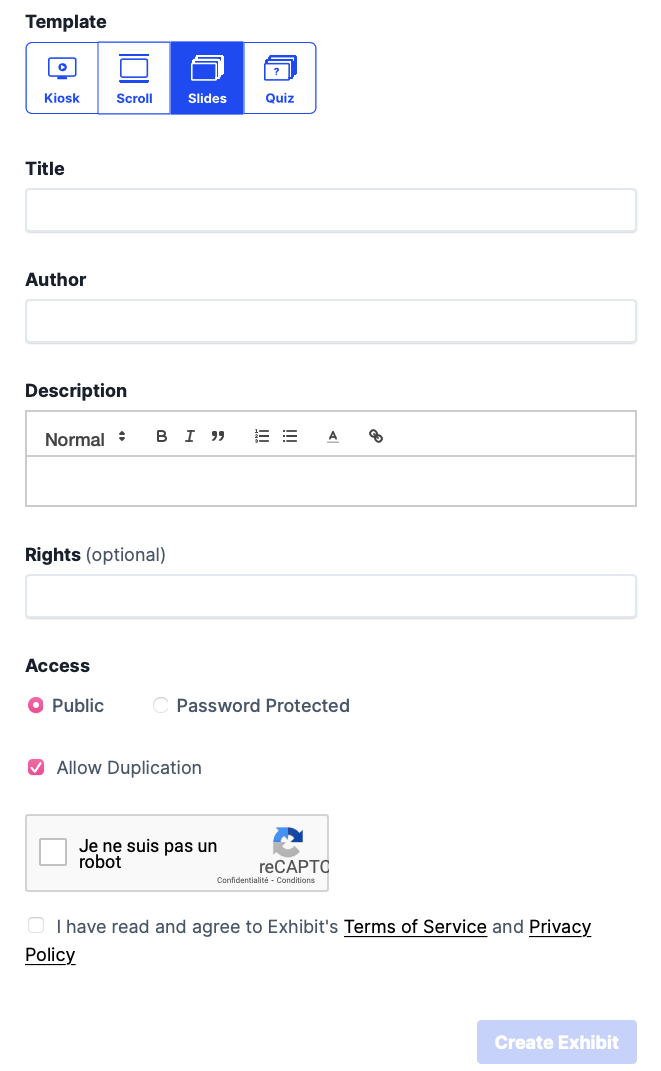
\includegraphics[scale=0.5, angle=0]{images/partie3/exhibit/exhibit-settings.png}
    \centering
    \end{figure}
    
    Avant de commencer à ajouter du contenu, il faut donc définir certains paramètres, en premier lieu le \textit{template}. Dans le cadre de l'exposition \textit{Medieval skies under(book)cover}, seul le \textit{template quiz} est utilisé. Il est ensuite nécessaire de définir un titre pour l'\textit{exhibit}, c'est le nom du parcours correspondant qui peut donc être utilisé. Un auteur et une description font aussi partie des éléments requis avant de pouvoir créer un \textit{exhibit}. 
    
	\subsubsection{Création de contenu grâce à cet outil} 
	Une fois l'\textit{exhibit} créé, du contenu peut y être intégré. Par contenu, on entend ici les \textit{attention points} du parcours que l'on souhaite ajouter. Comme précédemment précisé, il est possible d'ajouter plusieurs \textit{manifests}. Toutefois, il faut être vigilant à bien sélectionner le bon \textit{manifest} lorsque l'on veut ajouter des \textit{attention points} afin de pouvoir associer le texte rédigé en amont au folio correspondant. 
	
	\begin{figure}[h]
	\caption{Interface d'ajout d'un \textit{manifest}}
	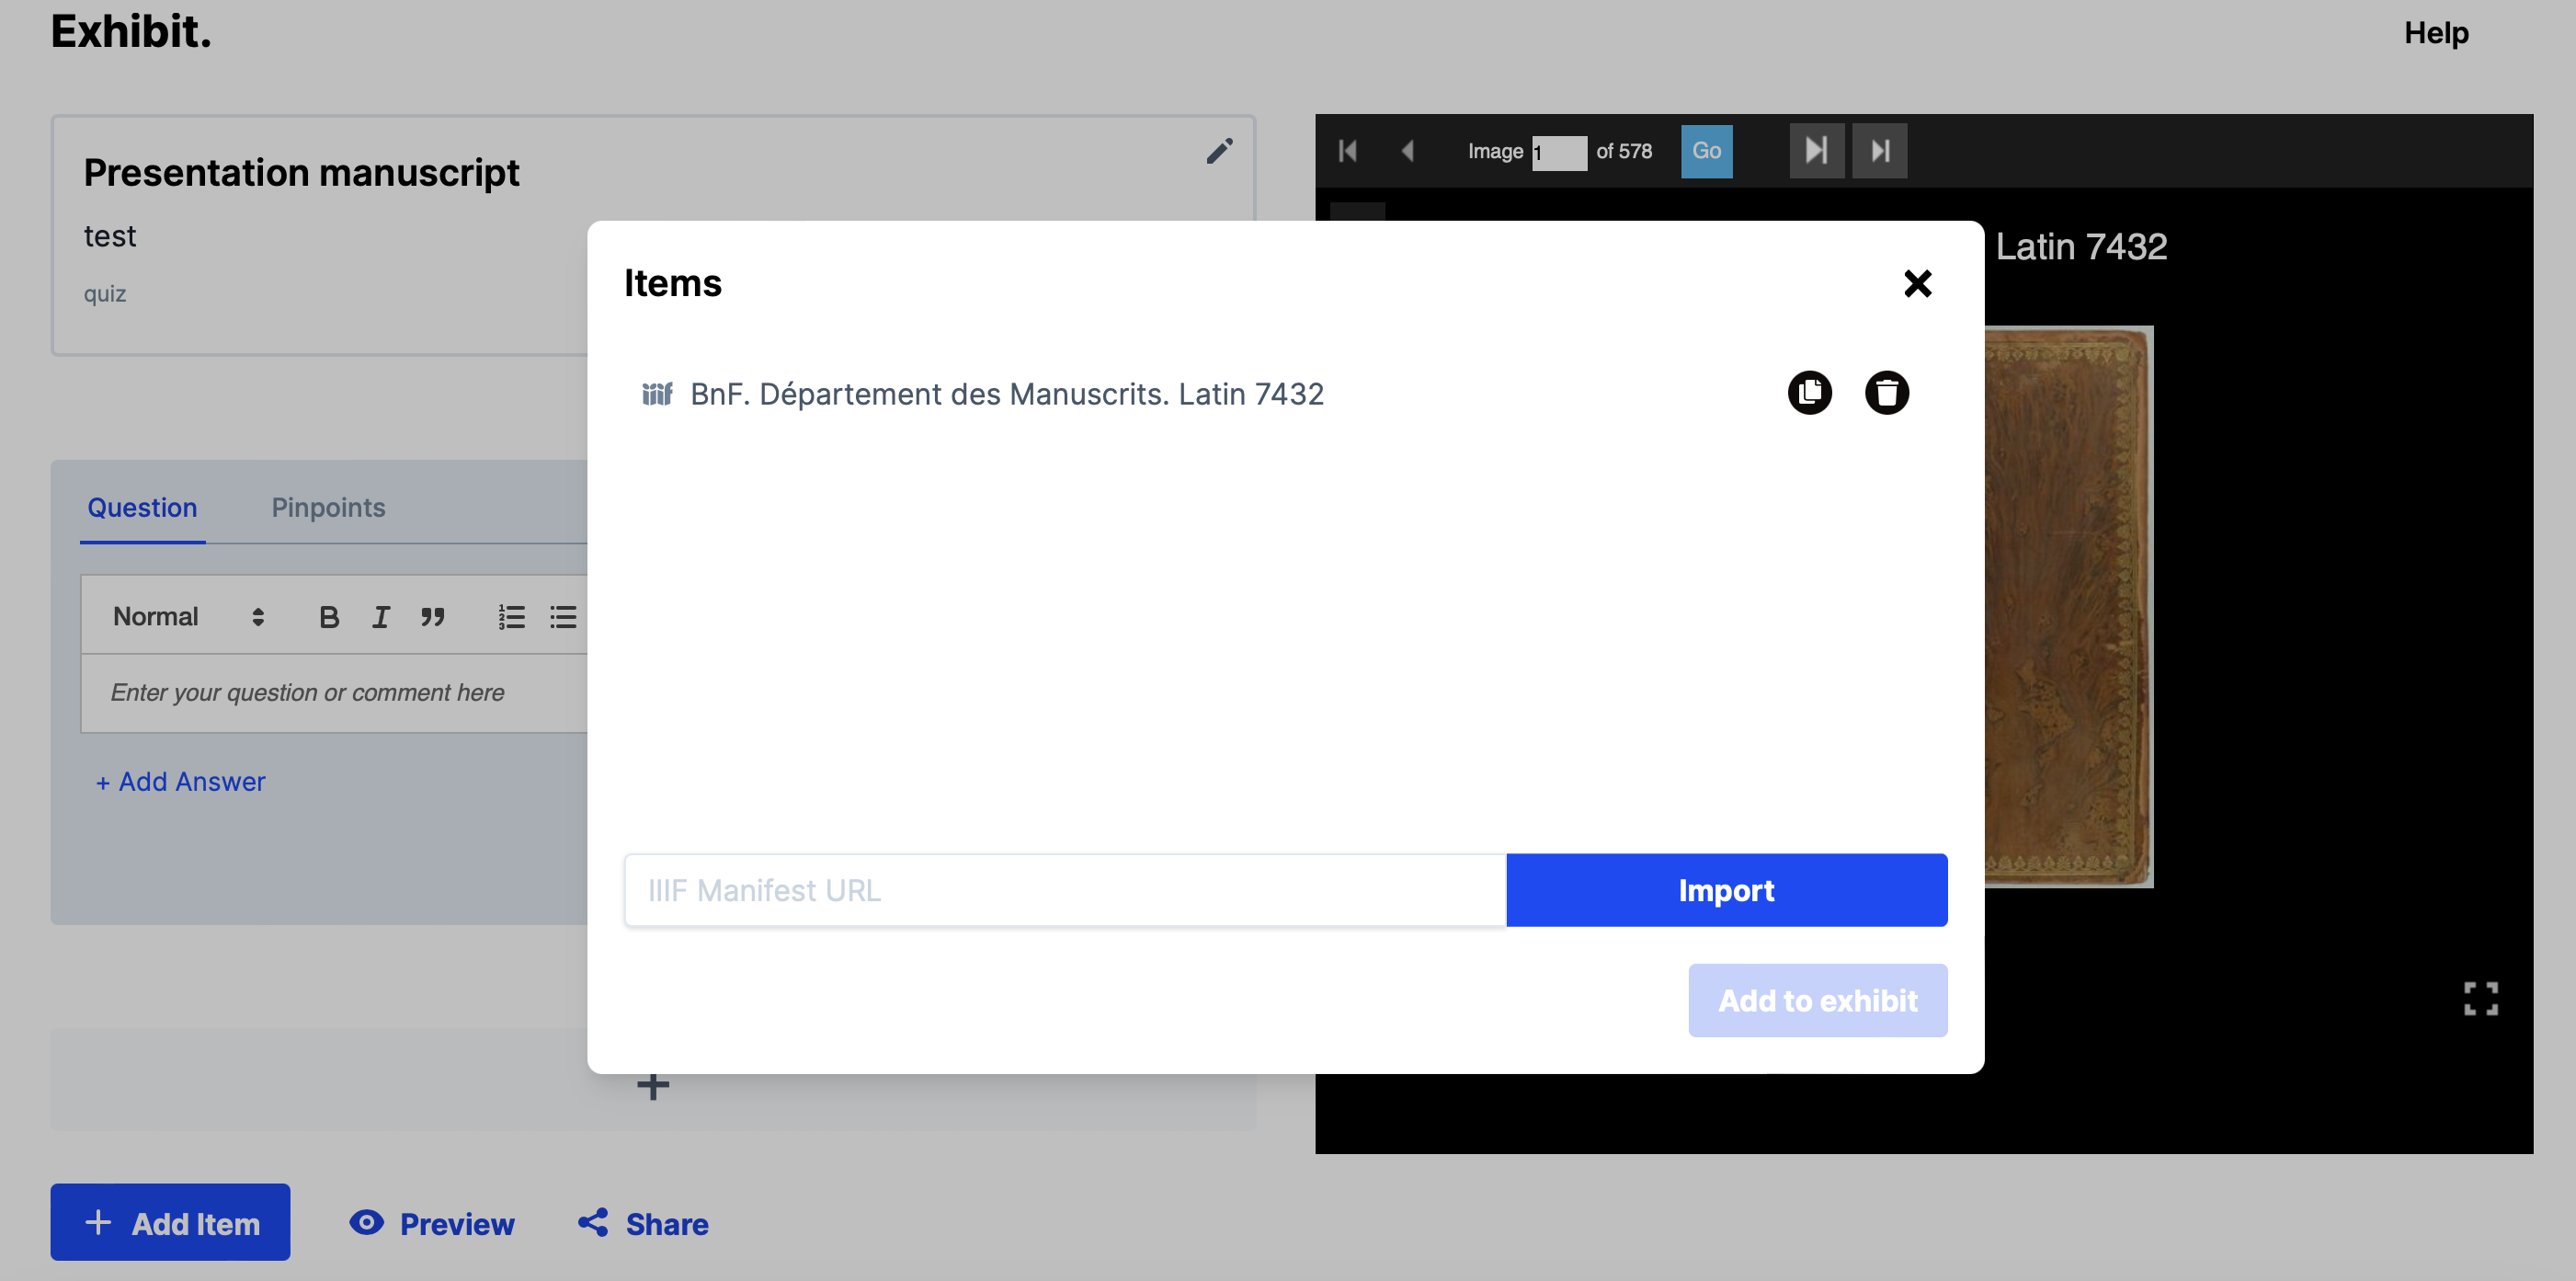
\includegraphics[scale=0.2, angle=0]{images/partie3/exhibit/exhibit-manifest.png}
    \centering
    \end{figure}
    
    
    \begin{figure}[h]
	\caption{Interface d'ajout de \textit{captions}}
	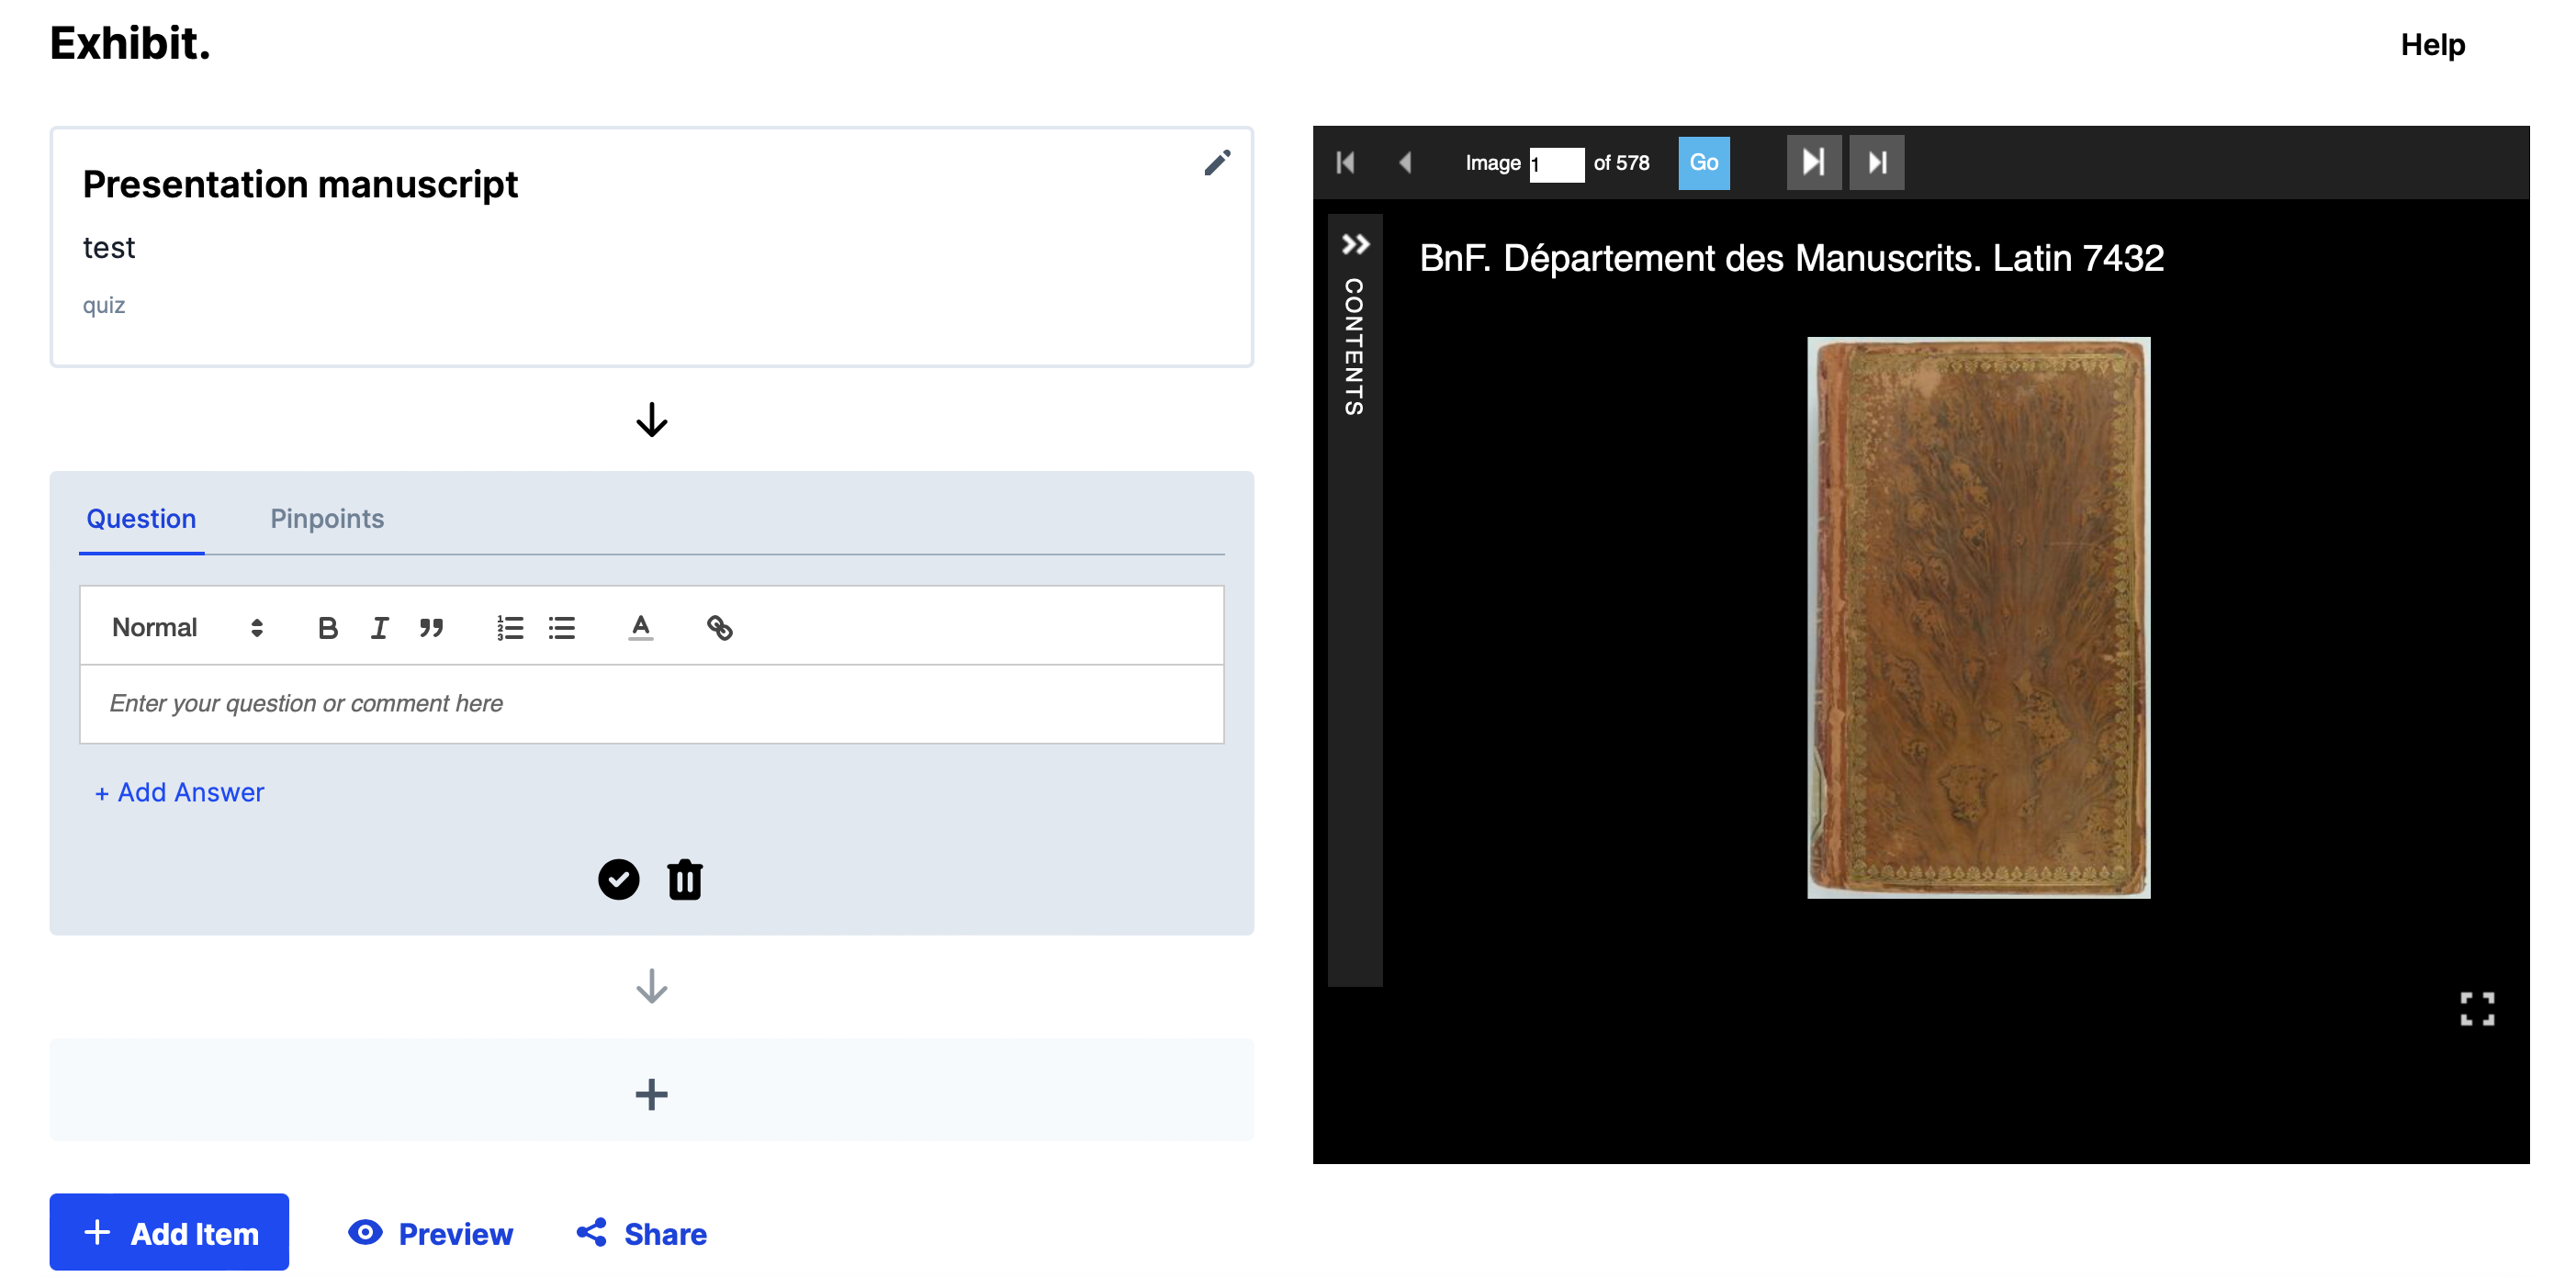
\includegraphics[scale=0.3, angle=0]{images/partie3/exhibit/exhbit-captions.png}
    \centering
    \end{figure}
    
    Sur l'interface d'Exhibit, les descriptions associées aux images sont appelées des \textit{captions}. C'est donc là que les \textit{attention points} sont recopiés et qu'ils vont pouvoir être mis en forme. En effet, il est possible de mettre des éléments en gras ou en italique pour souligner leur importance aux yeux du lecteur. C'est également dans cette interface que l'auteur pourra choisir le folio à associer et choisir, s'il le souhaite, de zoomer sur une partie précise de celui. Comme indiqué, pour plus de précisions encore, l'utilisation de \textit{pinpoints} est possible et c'est dans cette même interface que cela se fait. 
    
    Pour satisfaire les besoins de la scénographie, les \textit{attention points} ne sont pas toujours utilisés tels qu'ils ont été produits par les chercheurs. En effet, s'ils sont trop longs notamment ils peuvent être découpés en plusieurs \textit{captions}, chacune associée à un zoom qui est donc plus précis du folio liée à l'\textit{attention point} \footnote{Pour plus de précision concernant les transformations des \textit{attention points} lors de leur intégration aux \textit{exhibits}, voir annexe \ref{Tutoriel}, à la page \pageref{Tutoriel}.}. La création des \textit{exhibits} pour chacun des parcours thématiques et manuscrits et la formalisation de recommandations pour les phases de relecture par les chercheurs ont occupé une grande partie de mon stage à l'Observatoire. Néanmoins, les \textit{attention points} n'ont, pour la plupart, été intégrés que dans leur version initiale et il reviendra aux chercheurs de les retravailler pour mettre en lumière les éléments qui méritent de l'être. Par ailleurs, quand des parcours raccourcis seront ajoutés, les \textit{exhibits} devront de nouveau faire l'objet d'une relecture pour ajouter si nécessaire des liens permettant aux visiteurs de naviguer d'un \textit{shortcut} à un autre. 
    
	\subsubsection{Ajout de fonctionnalité}
	Évoquée au début de cette partie, la communauté \acrshort{iiif} est véritablement active et participative. Ainsi, prendre contact avec l'un des développeurs d'Exhibit, Edward Silverton, s'est fait sans encombre. L'objectif était alors de discuter de la possibilité d'ajouter une fonctionnalité à Exhibit : le \textit{deeplinking} ou la création de liens spécifiques à chaque \textit{slide} d'un \textit{exhibit}. En effet, jusqu'alors le lien renvoyait systématiquement au début. La perspective de ces liens plus précis représente un atout important pour le futur de l'exposition et la création de versions courtes pour certains parcours. Cette fonctionnalité a pu être implémentée rapidement, bien avant la fin du stage, ce qui a permis de la tester et de valider ainsi la proposition faite par Edward Silverton. Chaque \textit{slide} a donc désormais un identifiant qui lui est propre, à la fin de son url \acrshort{url}. 
	
	Cet ajout est déjà utilisé dans l'exposition pour le glossaire. En effet, dans celui-ci sont référencées toutes les mentions des différentes figures historiques au sein de l'exposition et pour chacune il a donc été possible d'indiquer le folio exact d'un manuscrit en renvoyant le visiteur avec précision vers la \textit{slide} concernée.

	
	\chapter{Élaboration de l’application web}
	Le présent chapitre est consacré au développement effectif de l'application web destinée à la visite de l'exposition \textit{Medieval skies under(book)cover}. Il y sera alors principalement question du code et de la manière dont il a été pensé et élaboré. 
	
	\section{Architecture de l’application flask}
	
    \subsection{Pages HTML}
    \subsubsection{\textit{Homepage}}
    \begin{figure}[h]
	\caption{Page d'accueil du site \textit{Medieval skies under(book)cover}}
	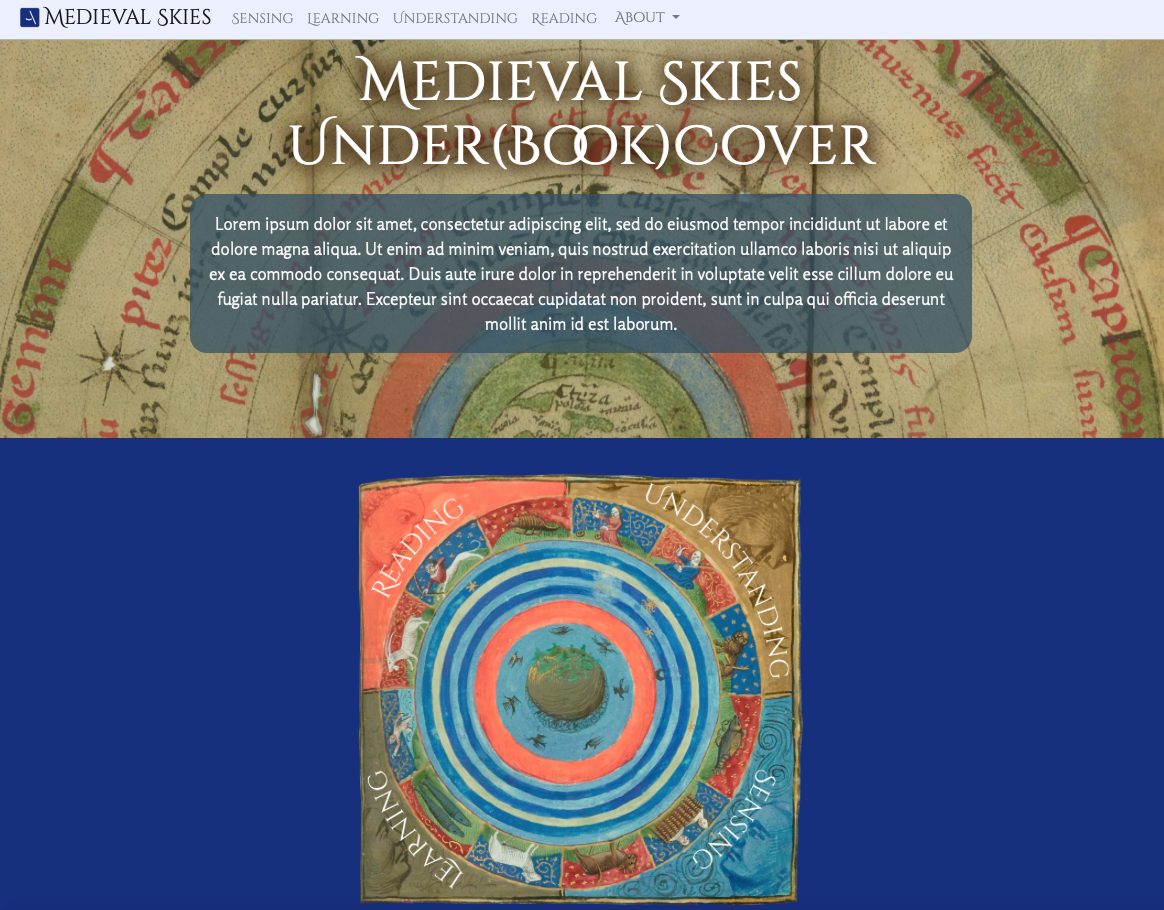
\includegraphics[scale=0.3, angle=0]{images/partie3/website/expo-homepage.png}
    \centering
    \end{figure}
    
    C'est ainsi que débute la visite de l'exposition. Dès le départ, le visiteur a donc face à lui des morceaux de manuscrits, l'une et l'autre des images choisies sont issus du manuscrit de présentation de Conrad Heingarter \footnote{Il s'agit du manuscrit Paris, BnF | Lat. 7432.}. Une description générale de l'exposition accompagnera bientôt le titre dans la partie haute de la page. La partie centrale est quant à elle interactive : les utilisateurs ont la possibilité de cliquer sur l'une des quatre parties\footnote{\textit{Sensing} renvoie aux parcours patrimoniaux, \textit{Learning} à ceux liés à l'histoire de l'astronomie alphonsine, \textit{Understanding} à ceux qui expliquent les notions scientifiques et \textit{Reading} à ceux qui mettent en lumière les manuscrits un à un.} de l'image, où sont représentés des vents, pour accéder au thème indiqué sur la partie choisie. Ces quatre thèmes sont également accessibles en cliquant sur le nom souhaité dans la barre de navigation. Grâce à cette même \textit{navbar}, la page d'accueil est accessible depuis toutes les pages du site web en cliquant sur le titre dans une version raccourcie, \textit{Medieval skies}. Cela respecte les attentes notées dans le document de spécification. Que le visiteur choisisse la barre de navigation ou la miniature interactive, une très brève description des thèmes est affichée au survol avec la souris, permettant de le guider dans son choix. Plus bas, la possibilité est offerte aux visiteurs de se rendre directement sur la page d'un des parcours désignés comme étant à voir absolument. Enfin, le pied de page, commun à l'ensemble du site web, permet de connaître les principaux partenaires et d'accéder à leurs propres sites web par un clic sur le logo. 
    
    \subsubsection{\textit{Themes}}
    Après avoir choisi un thème à visiter, l'utilisateur découvre l'une de ces quatre pages \footnote{Elles sont accessibles : \href{https://alfa-exhibition.herokuapp.com/heritage}{\textit{Sensing}}, \href{https://alfa-exhibition.herokuapp.com/historical}{\textit{Learning}}, \href{https://alfa-exhibition.herokuapp.com/scientific}{\textit{Understanding}} et \href{https://alfa-exhibition.herokuapp.com/manuscripts}{\textit{Reading}}.}, chacune construite selon le même principe. 
    
    \begin{figure}[!h]
    \centering
    \begin{subfigure}[h]{0.4\textwidth}
        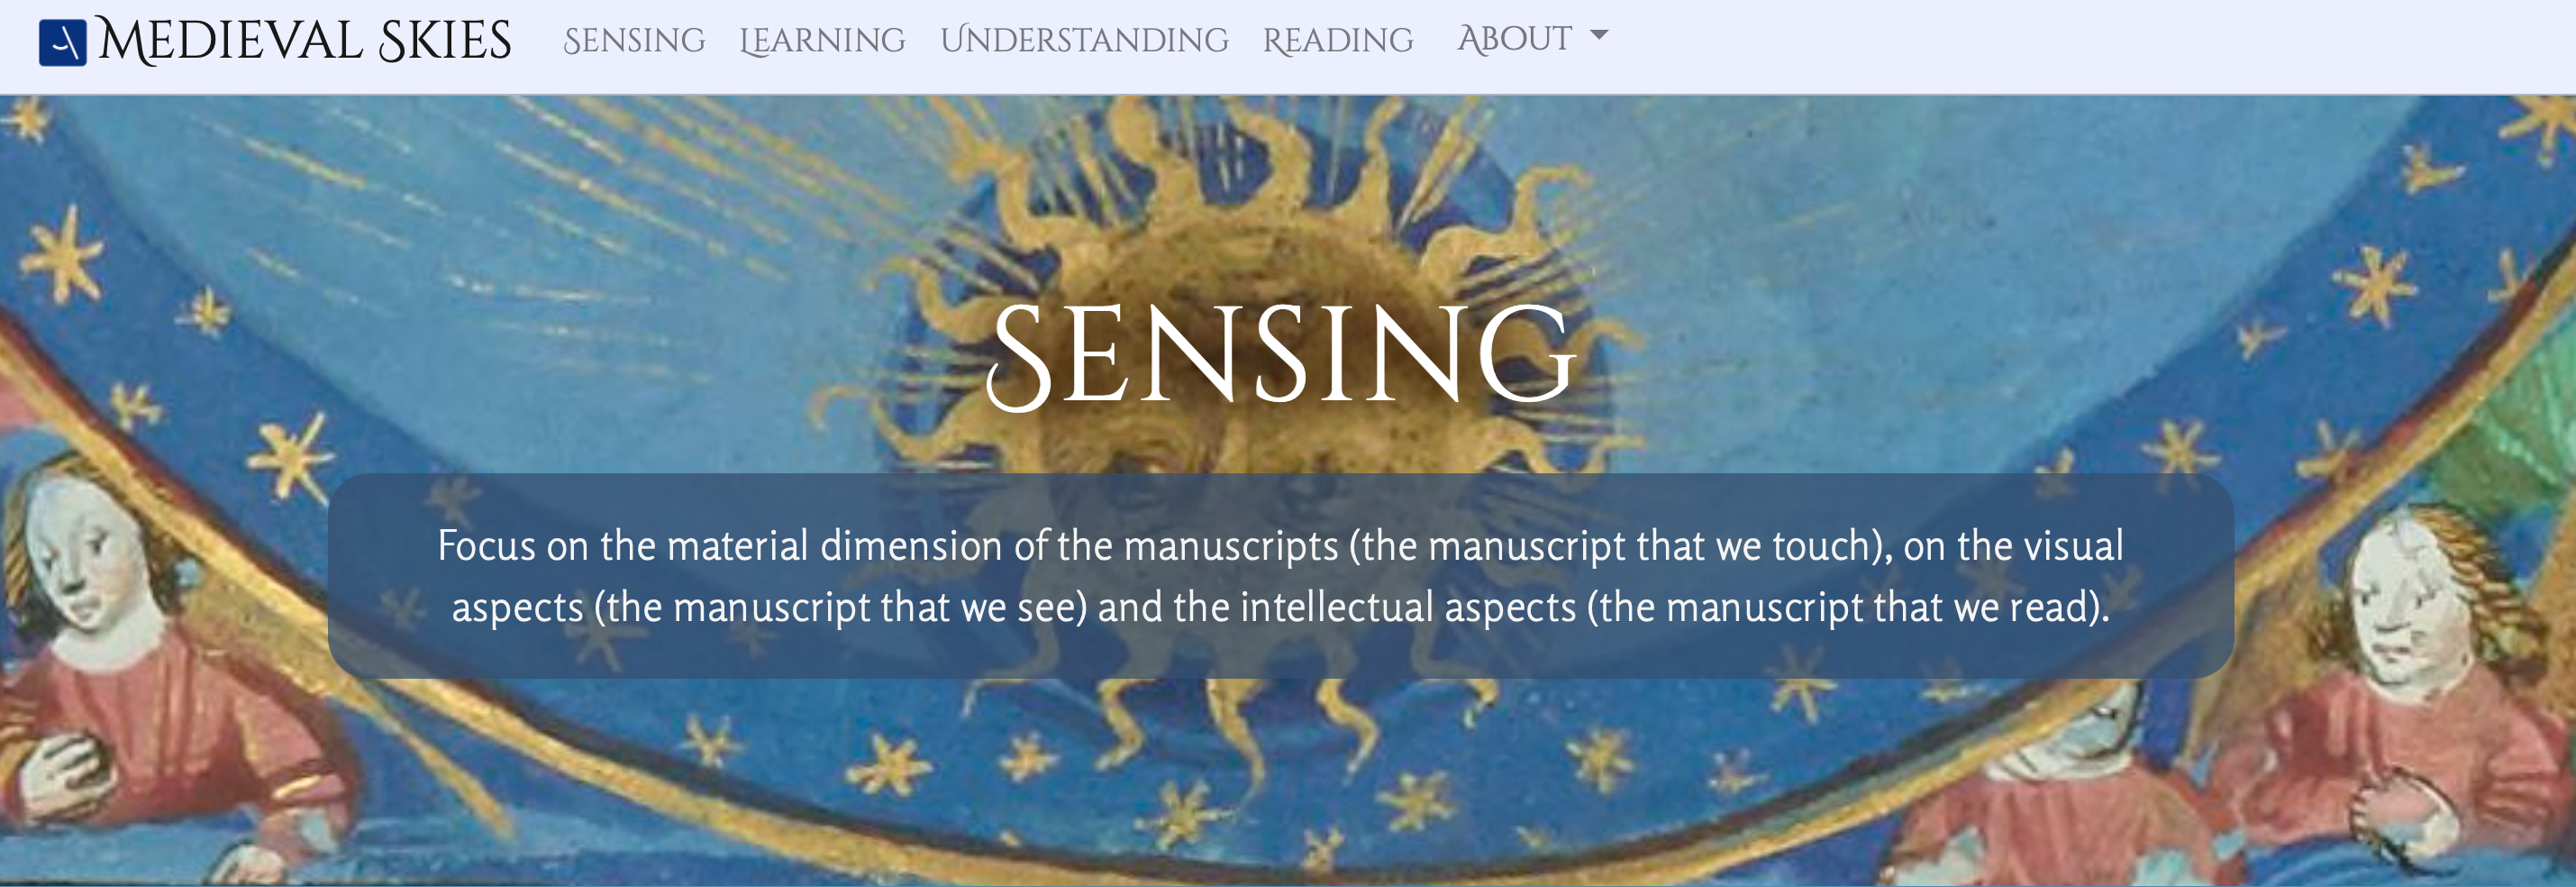
\includegraphics[width=\textwidth]{images/partie3/website/expo-sensing.png}
    \end{subfigure}
    \begin{subfigure}[h]{0.4\textwidth}
        \includegraphics[width=\textwidth]{images/partie3/website/expo-learning.png}
    \end{subfigure}
    \begin{subfigure}[h]{0.4\textwidth}
        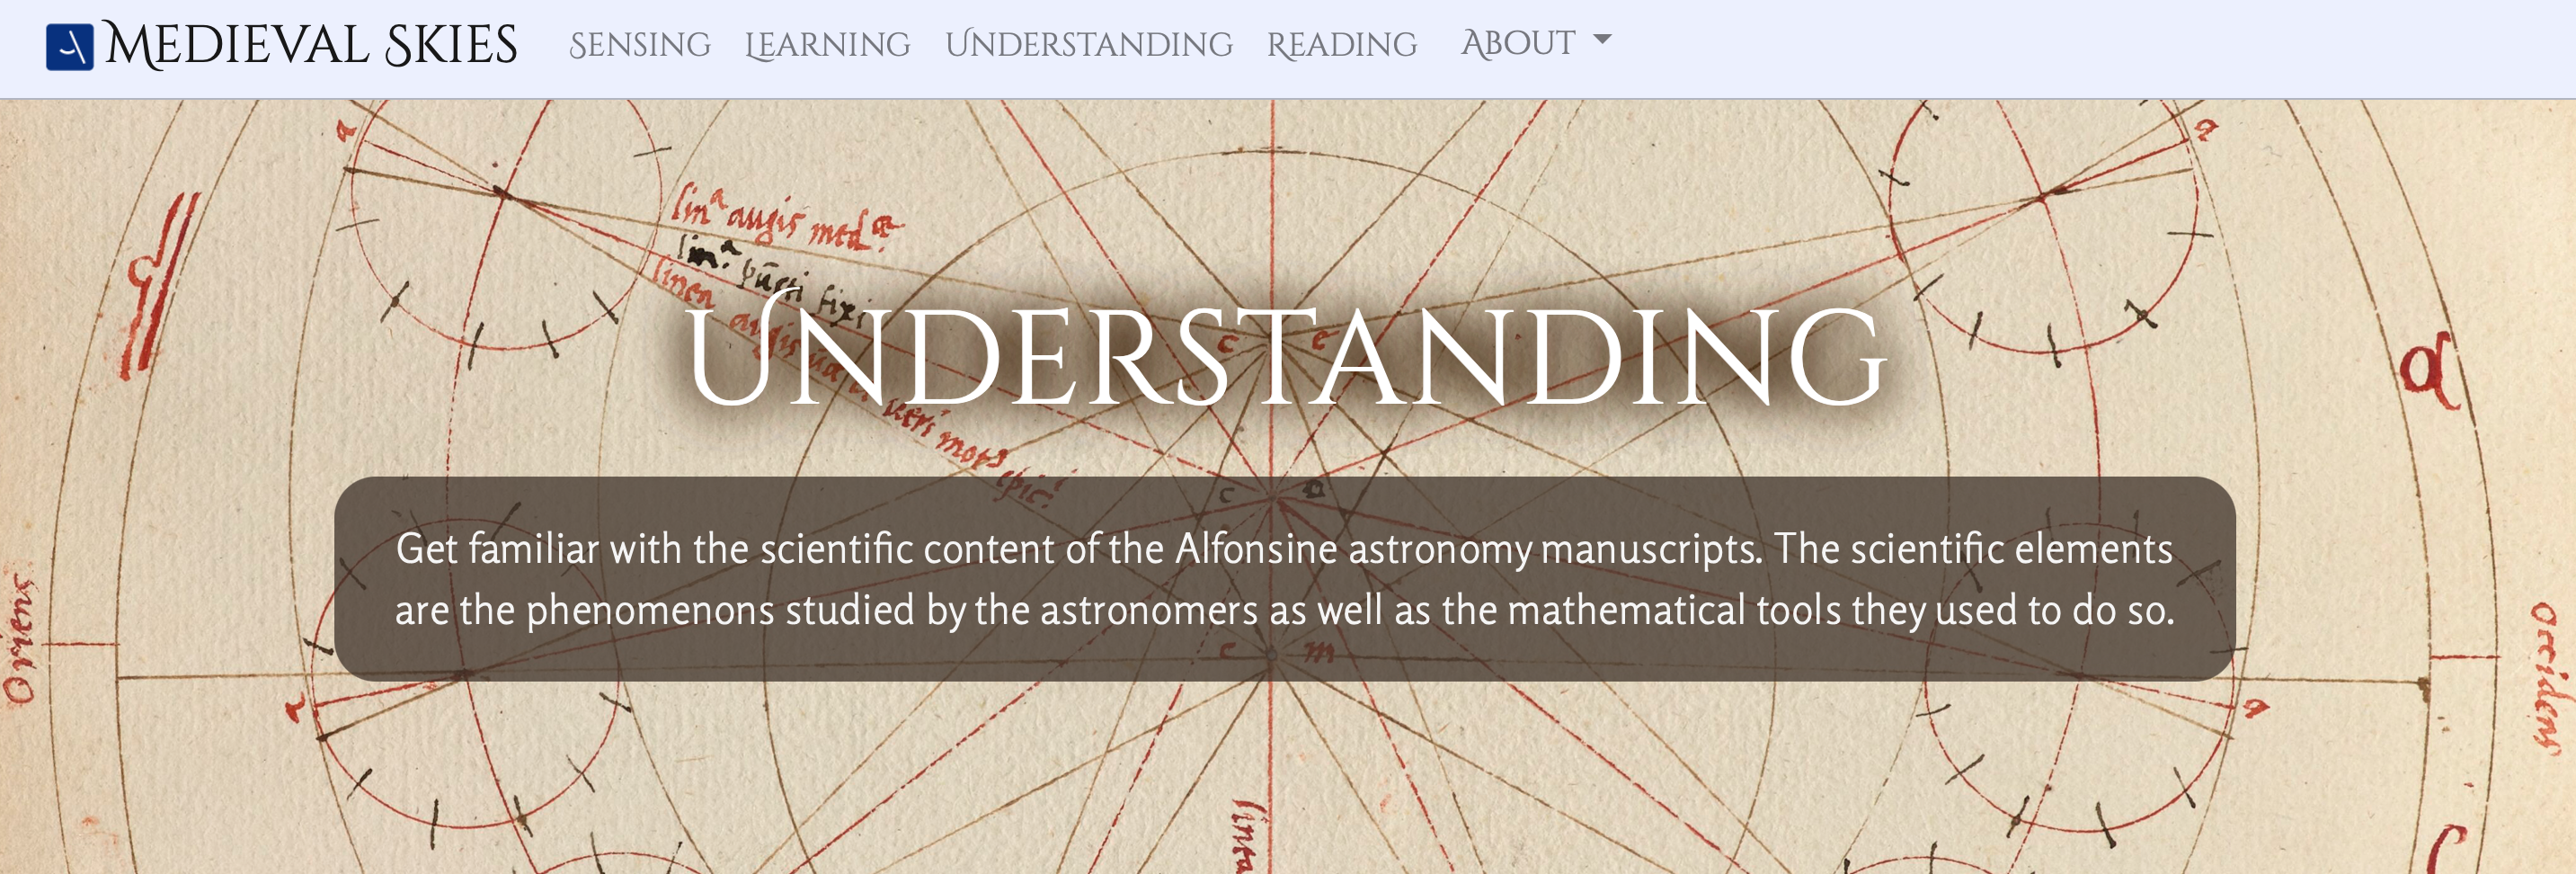
\includegraphics[width=\textwidth]{images/partie3/website/expo-understanding.png}
    \end{subfigure}
    \begin{subfigure}[h]{0.4\textwidth}
        \includegraphics[width=\textwidth]{images/partie3/website/expo-reading.png}
    \end{subfigure}
    \caption{Pages \textit{Sensing}, \textit{Learning}, \textit{Understanding} et \textit{Reading} du site \textit{Medieval skies under(book)cover}}
    \end{figure}

    Les captures d'écran présentées ici correspondent à la partie supérieure de chacune de ces pages. On peut remarquer que la \textit{navbar} est toujours présente. Sous le titre des thèmes, une description plus longue du contenu est proposée afin d'aiguiller les visiteurs. Les images choisies proviennent à chaque fois d'un manuscrit exposé dans au moins un des parcours du thème choisi. 
    
    Plus bas sur chacune de ces pages, le visiteur a le choix parmi les différents parcours qui composent le thème où il se trouve.
    
    \begin{figure}[h]
	\caption{Page \textit{Reading} du site \textit{Medieval skies under(book)cover}}
	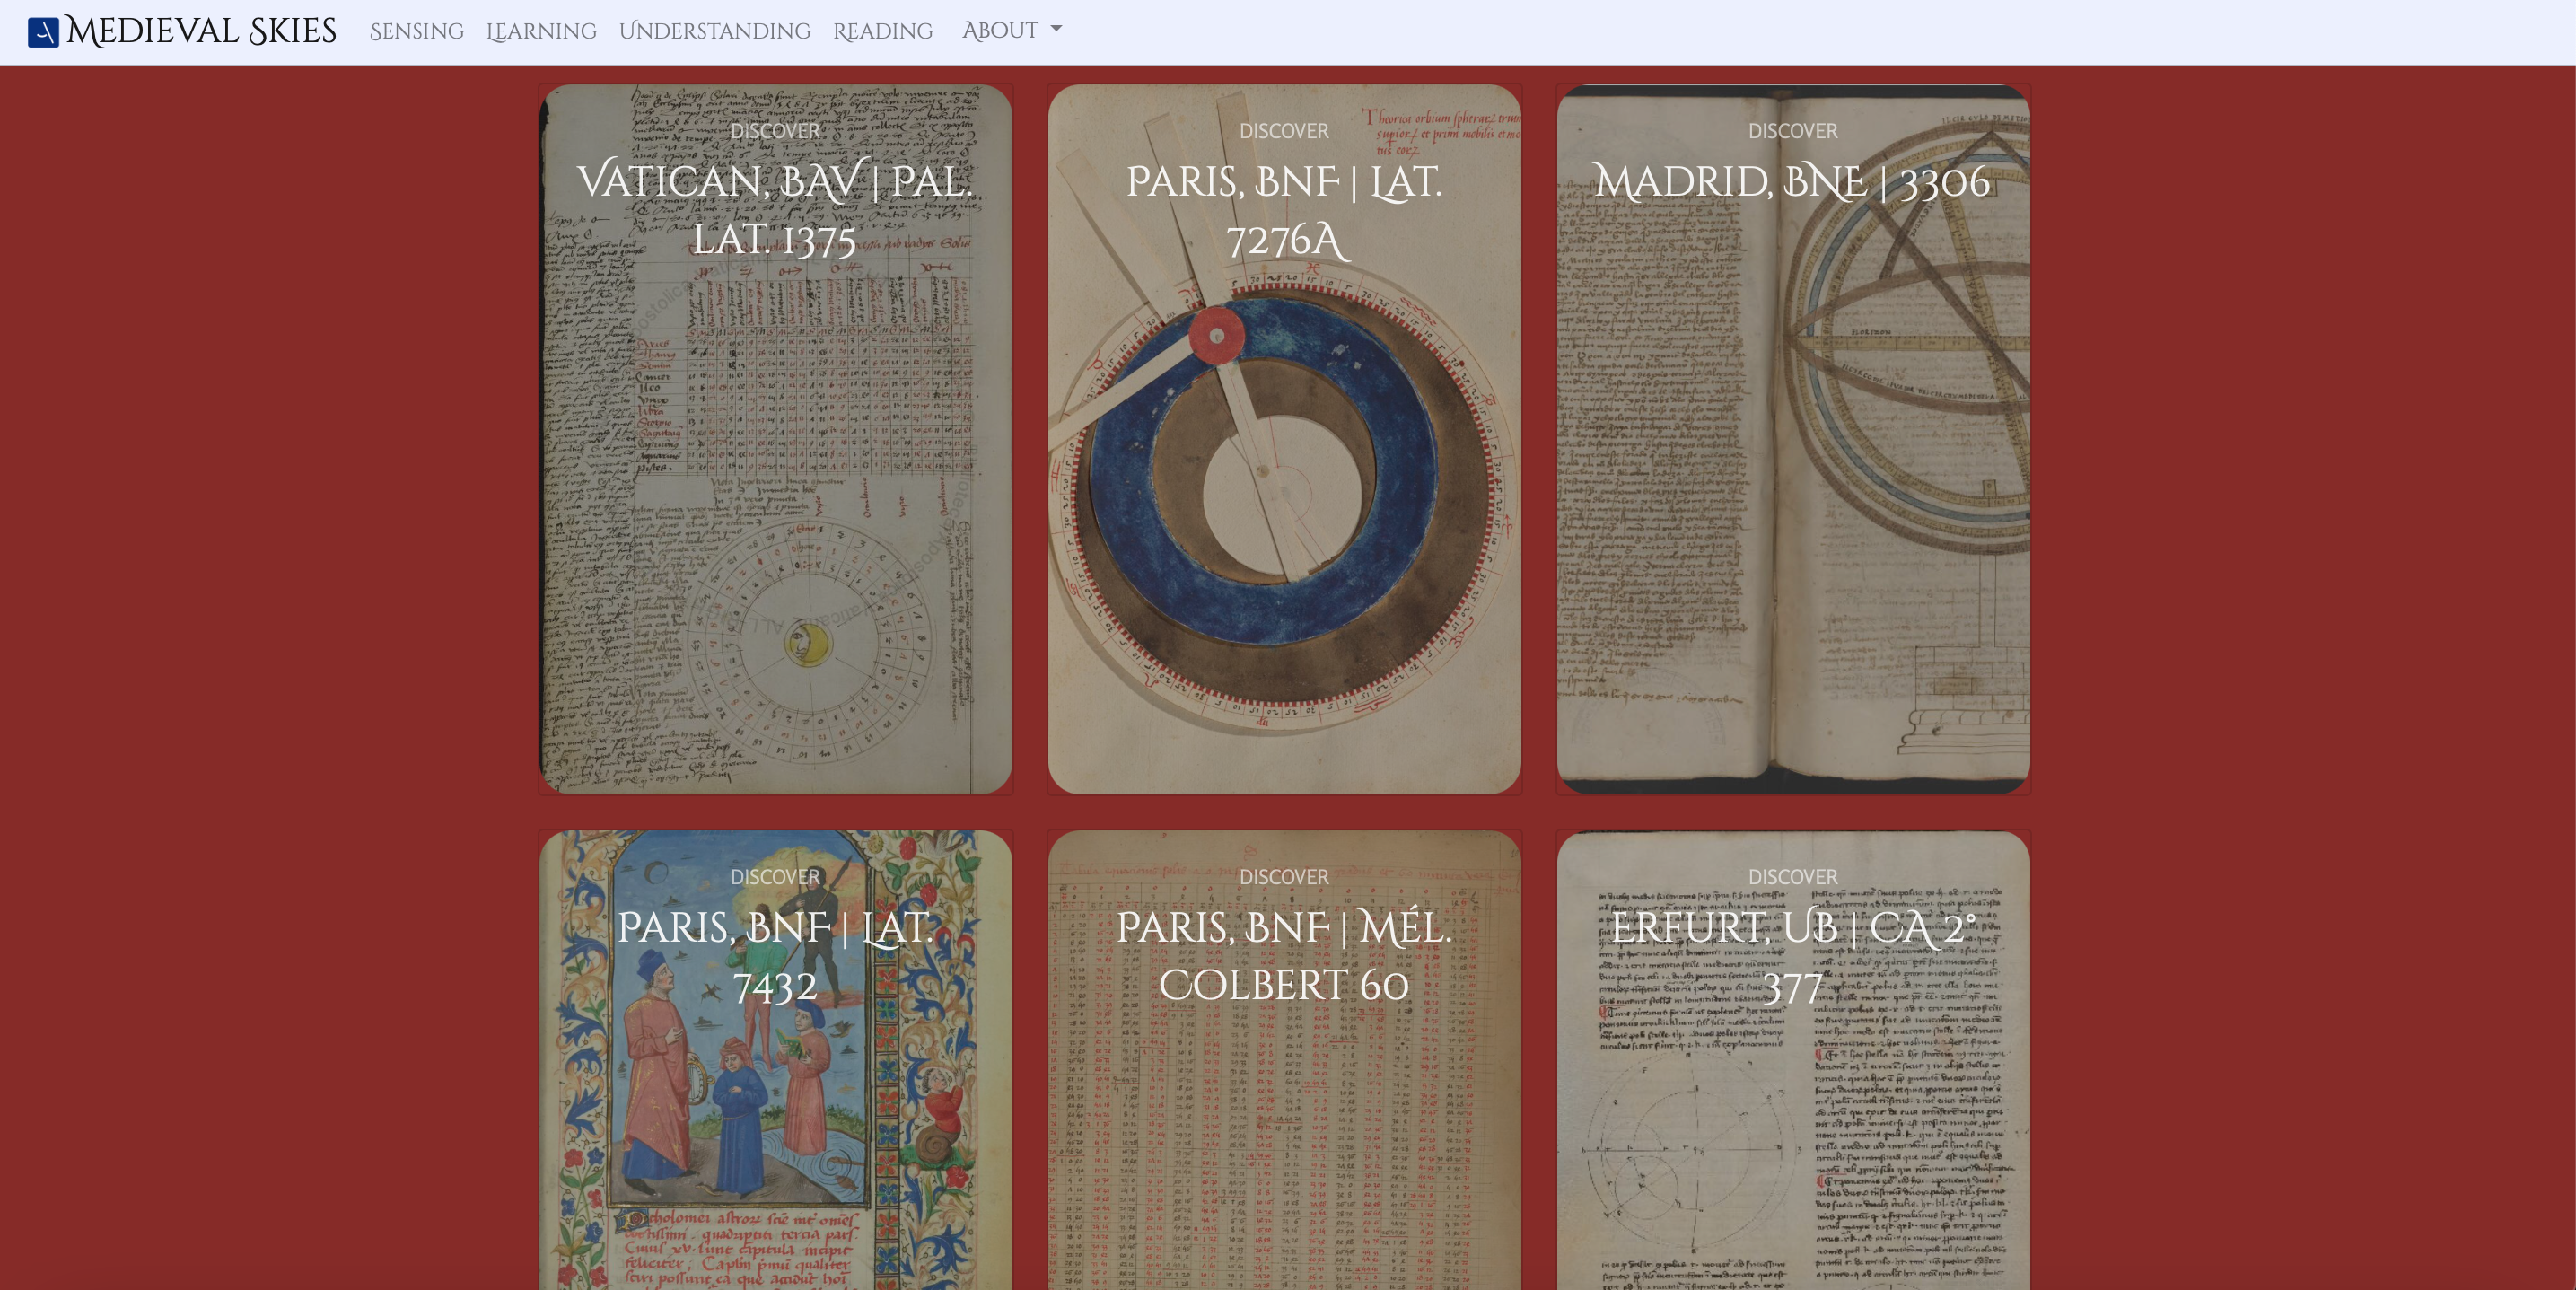
\includegraphics[scale=0.3, angle=0]{images/partie3/website/expo-reading-cards.png}
    \centering
    \end{figure}
    
    Seul est ici pris l'exemple du thème \textit{Reading} mais l'organisation est presque identique sur chacune des quatre pages : la seule différence étant le nombre de parcours, et donc de cartes cliquables, disponibles.
    
    Enfin, en bas de chacune de ces pages, le visiteur a à sa disposition un carrousel qui lui permet d'accéder aux trois autres thèmes depuis celui où il se trouve.  Prenons l'exemple de la page dédiée aux aspects patrimoniaux :
    
    \begin{figure}[h]
	\caption{Page \textit{Sensing} du site \textit{Medieval skies under(book)cover}}
	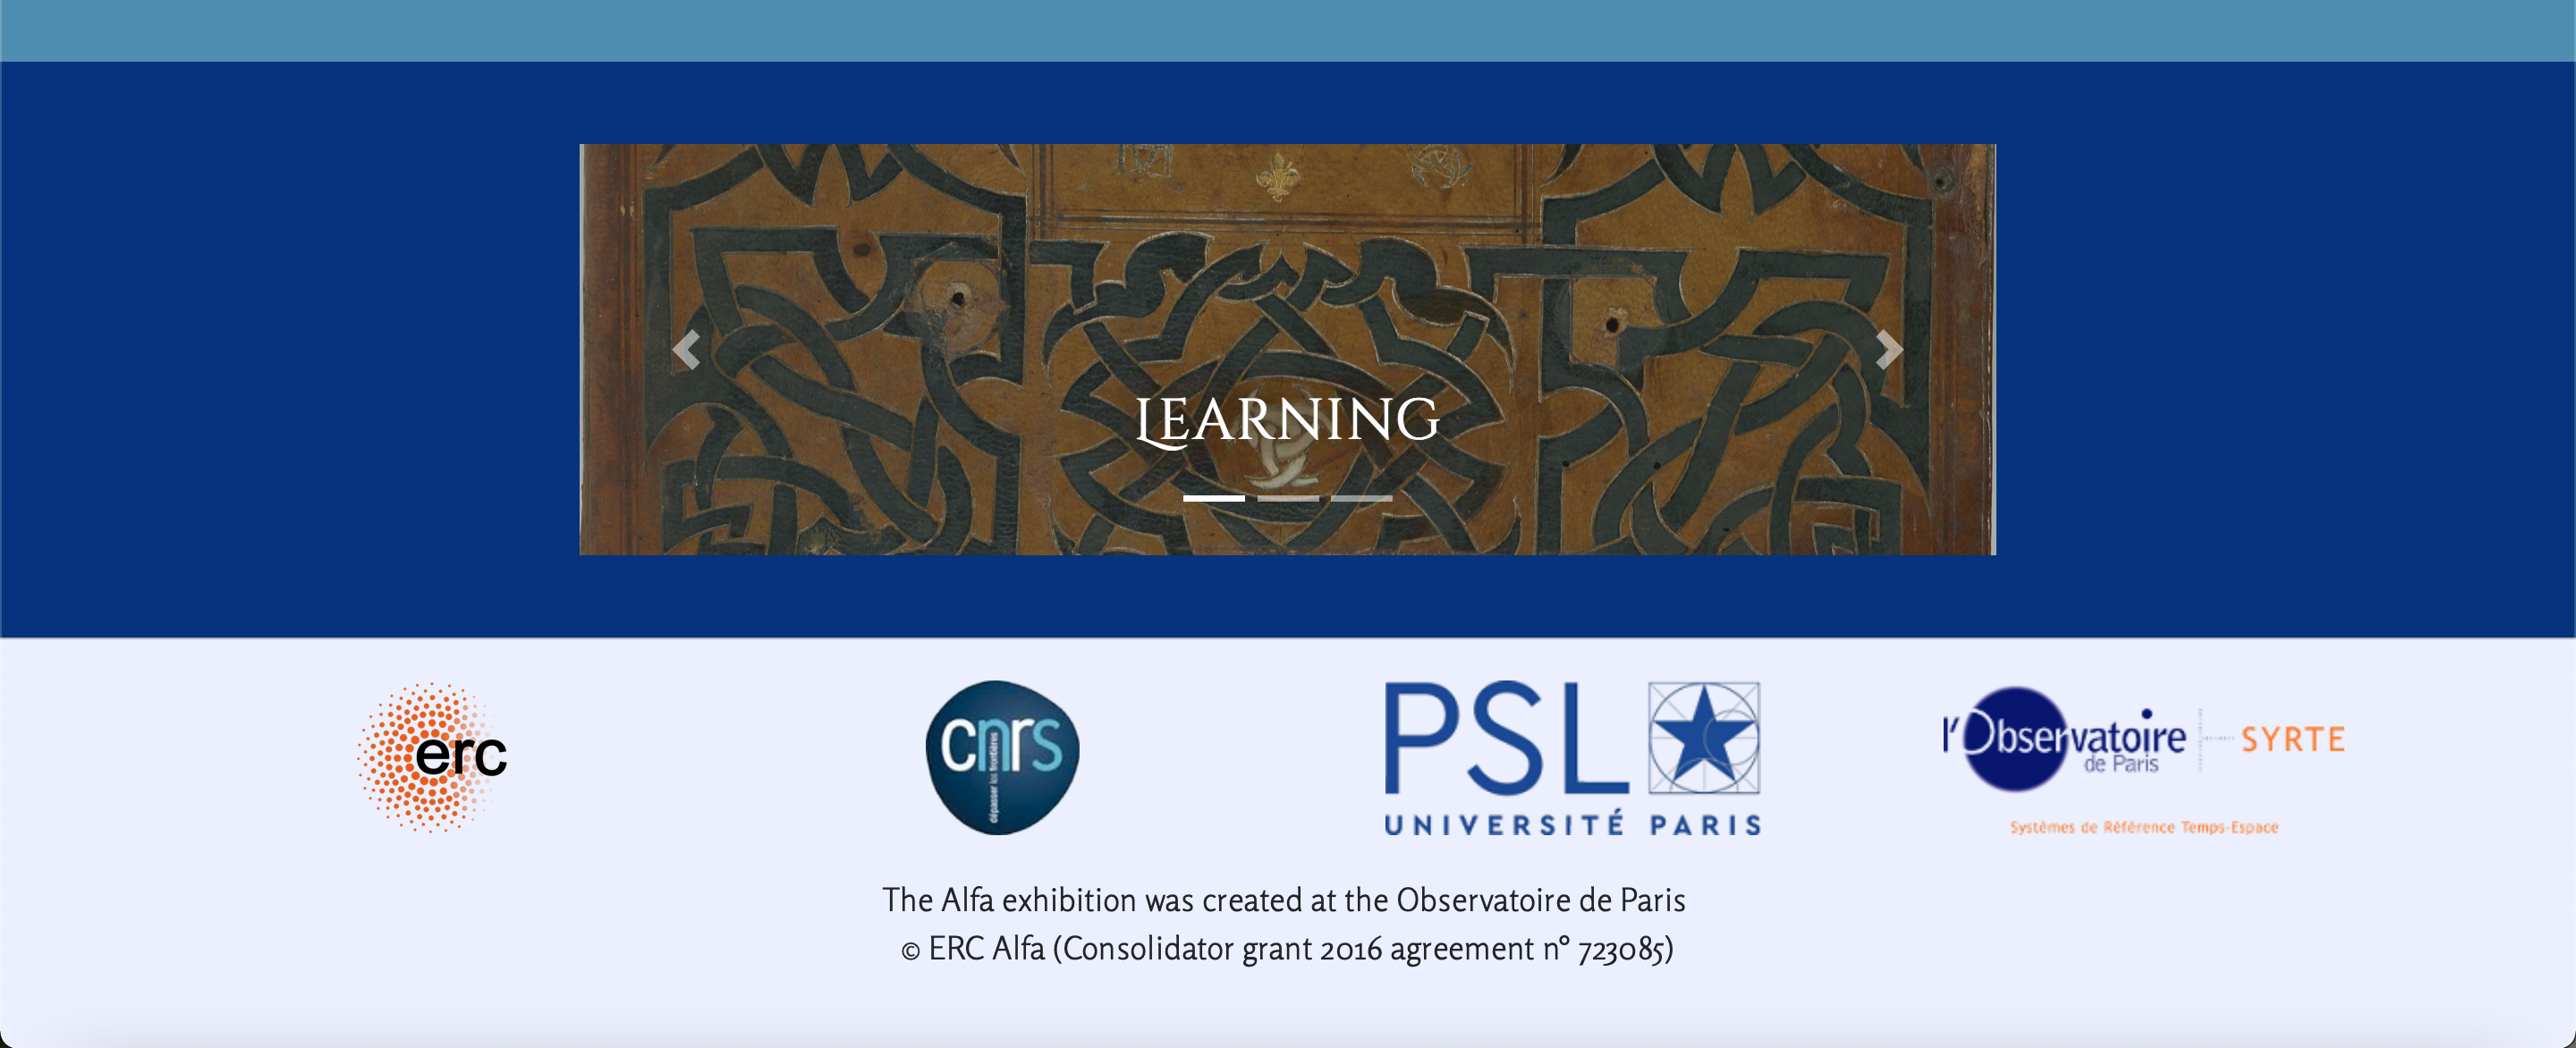
\includegraphics[scale=0.3, angle=0]{images/partie3/website/expo-sensing-carrousel.png}
    \centering
    \end{figure}
    
    On peut remarquer que l'image utilisée, ici pour le thème \textit{Learning} est la même qu'au début de la page de ce thème : c'est un autre moyen de guider les utilisateurs, en maintenant un cadre cohérent où ils peuvent se repérer aisément. 
    
    \subsubsection{\textit{Paths}}
    Pour accéder au parcours de son choix, le visiteur est appelé à cliquer sur la carte qui correspond à celui-ci. Là encore, tous les parcours se présentent de la même manière donc un unique exemple sera pris pour illustrer ce type de page.
    
    \begin{figure}[h]
	\caption{Page \textit{Exceptional manuscript} du site \textit{Medieval skies under(book)cover}}
	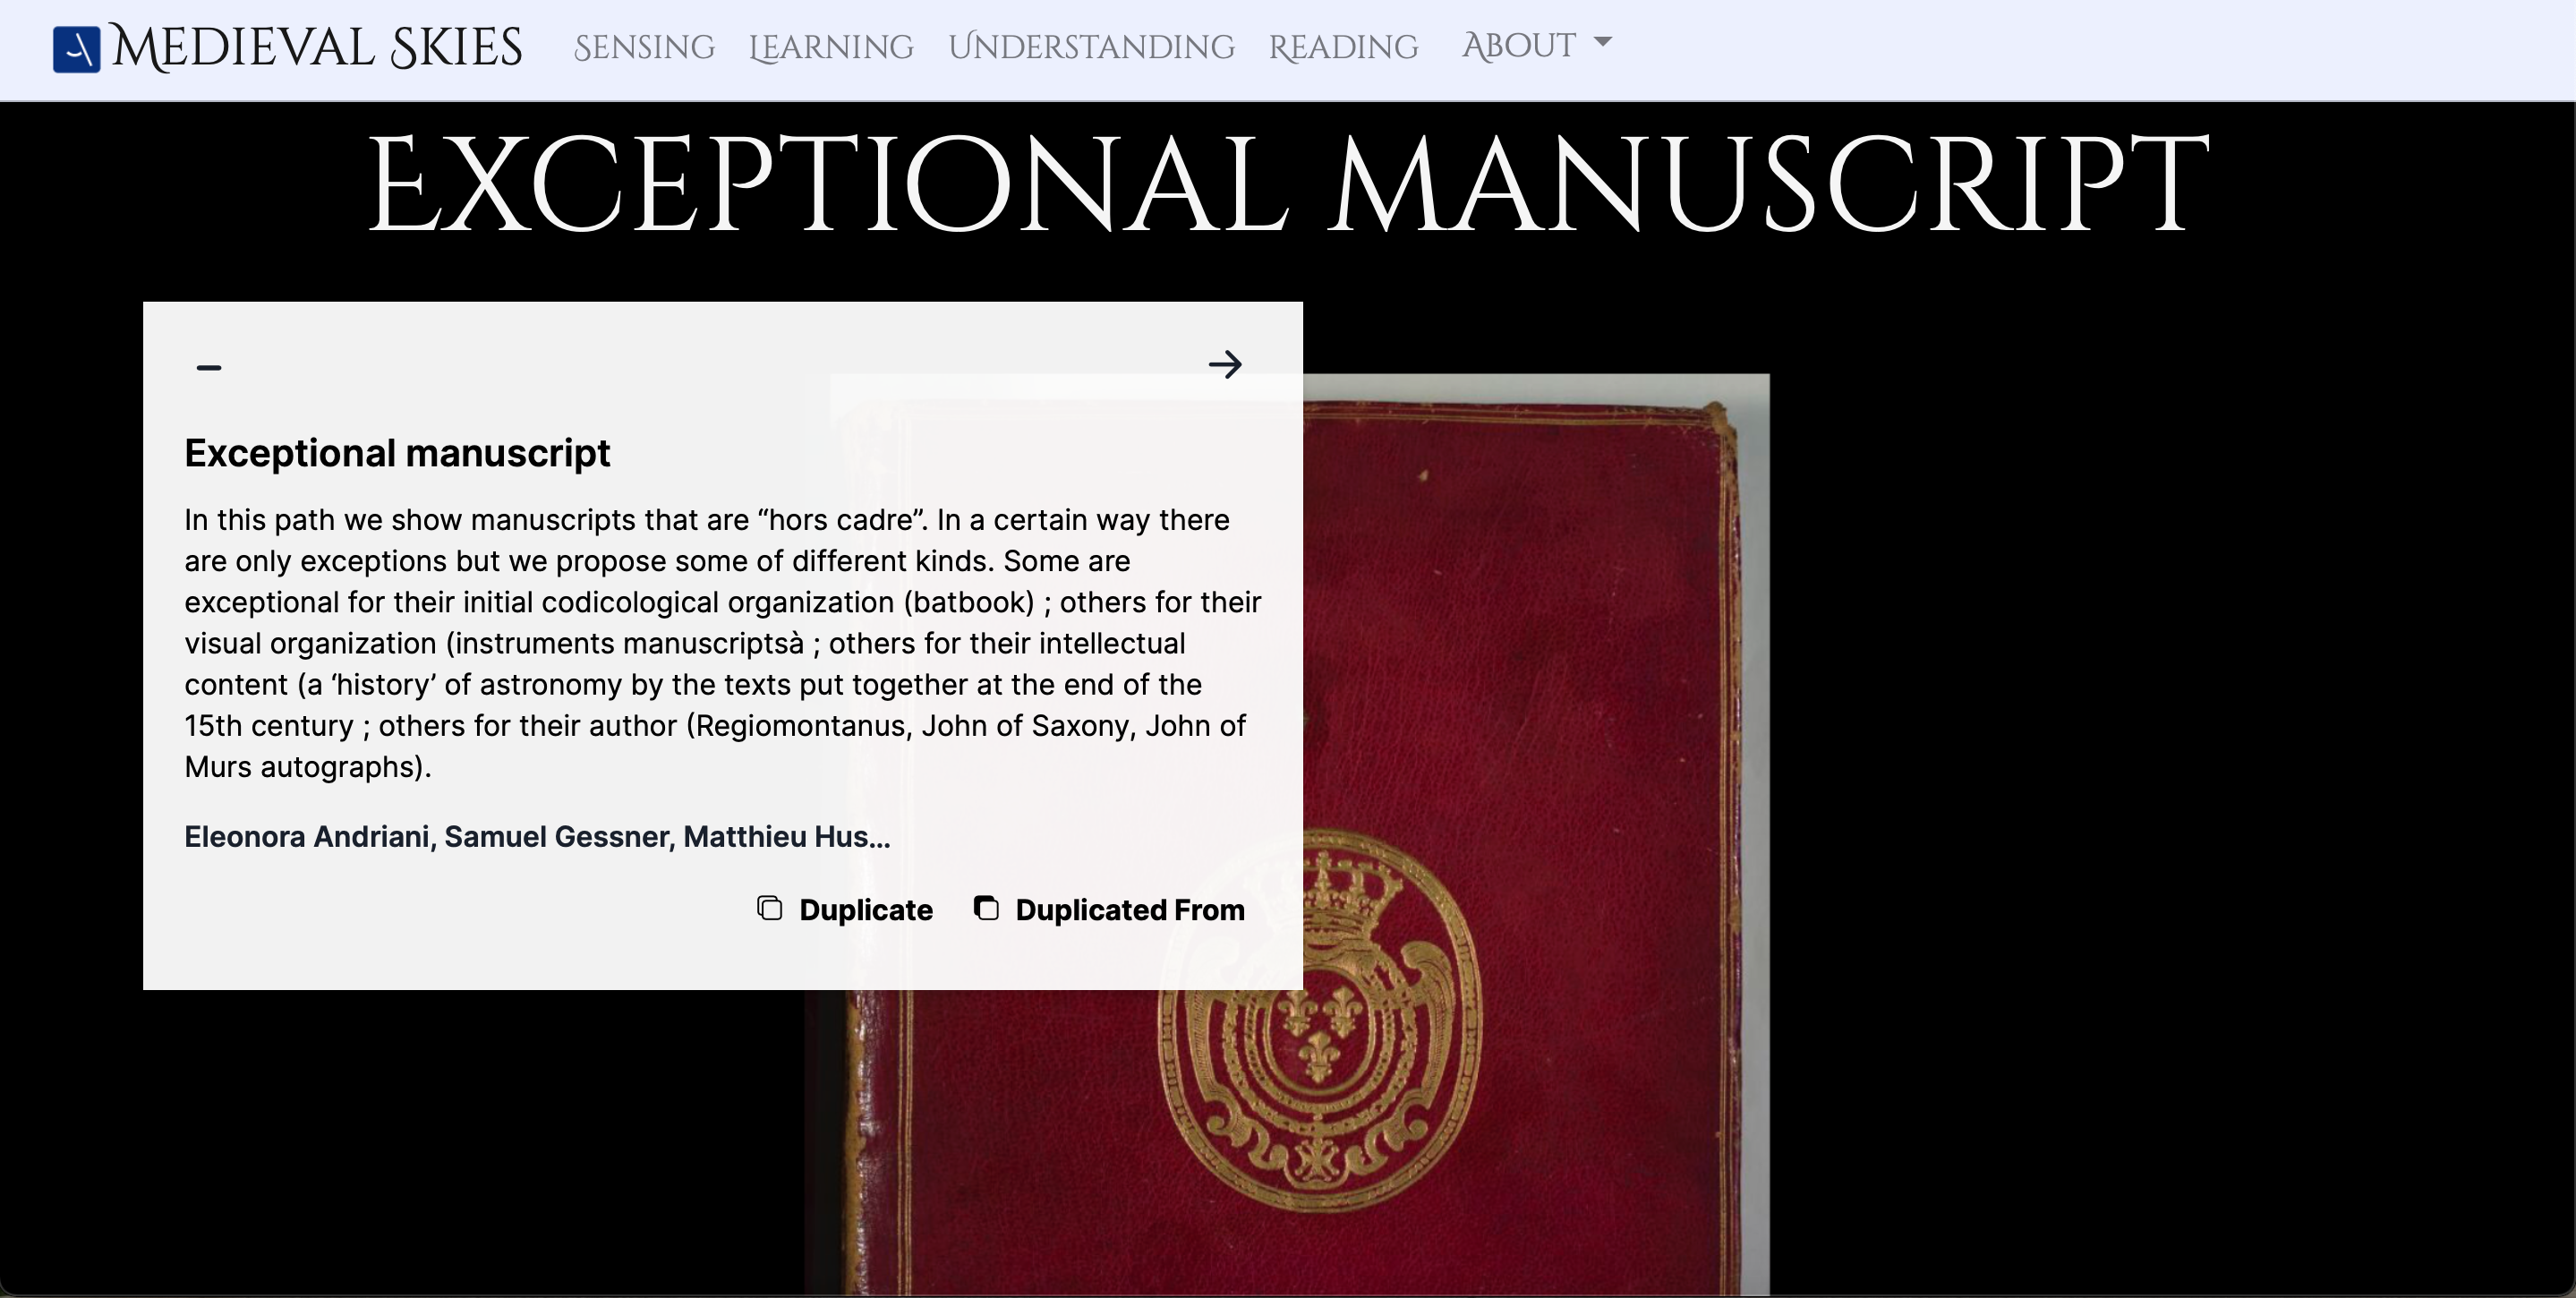
\includegraphics[scale=0.3, angle=0]{images/partie3/website/expo-paths-exceptional.png}
    \centering
    \end{figure}
    
    Outre la \textit{navbar} qui est toujours présente. Le visiteur accède ici à l'\textit{exhibit} créé pour ce parcours selon la méthode évoquée au précédent chapitre. Il peut ainsi découvrir les \textit{attention points} définis par les chercheurs. Une fois ce parcours terminé, il peut accéder aux autres parcours du même thème par le biais d'un carrousel en bas de page, de la même manière que ce qui a été montré pour les pages relatives aux quatre grands thèmes.
    
    \subsubsection{\textit{About}}
    Un élément de la \textit{navbar} n'a pas encore été évoqué : \textit{About}. C'est un menu déroulant qui permet d'accéder à trois autres pages qui ne contiennent pas de contenu directement inclus dans l'exposition. Ces pages sont les suivantes : \textit{About this project}, \textit{Glossary} et \textit{Bibliography} \footnote{Elles sont également accessibles : \href{https://alfa-exhibition.herokuapp.com/about}{\textit{About this project}}, \href{https://alfa-exhibition.herokuapp.com/glossary}{\textit{Glossary}} et \href{https://alfa-exhibition.herokuapp.com/bibliography}{\textit{Bibliography}}}. Ces pages ne sont pas encore finalisées : leur contenu doit être rédigé par l'équipe scientifique mais la structure est, elle, déjà en place. 
    
    Pour la page \textit{About this project}, l'idée est d'avoir une première section donnant aux visiteurs des précisions sur le projet \acrshort{alfa} au delà de l'exposition puis d'avoir un \textit{listing} des membres de l'équipe avant de terminer par quelques mots sur les institutions qui conservent les manuscrits utilisés dans cette exposition. 
    
    La page \textit{Bibliography} est la plus incomplète. Comme son nom le suggère, y seront renseignés des éléments bibliographiques qui permettront aux divers visiteurs d'accéder à des ressources complémentaires, plus précises et externes à l'exposition. Une seule référence est à ce jour visible dans le but de faire un test. Cela fait partie des éléments qui seront à compléter par l'équipe scientifique mais là encore, l'architecture de la page est prévue.
    
    Enfin, la page \textit{Glossary} qui, bien qu'incomplète, est la plus avancée des trois. C'est une sorte de répertoire des figures historiques : les liens des \textit{attention points} de l'exposition qui font mention de ces différents personnages y sont reportés, de même que ceux des notices Wikipedia et Biblissima, quand ces ressources existent. Les biographies qui viendront compléter ces références devront, quant à elle, être rédigées.
    
    \begin{figure}[!h]
    \centering
    \begin{subfigure}[h]{0.5\textwidth}
        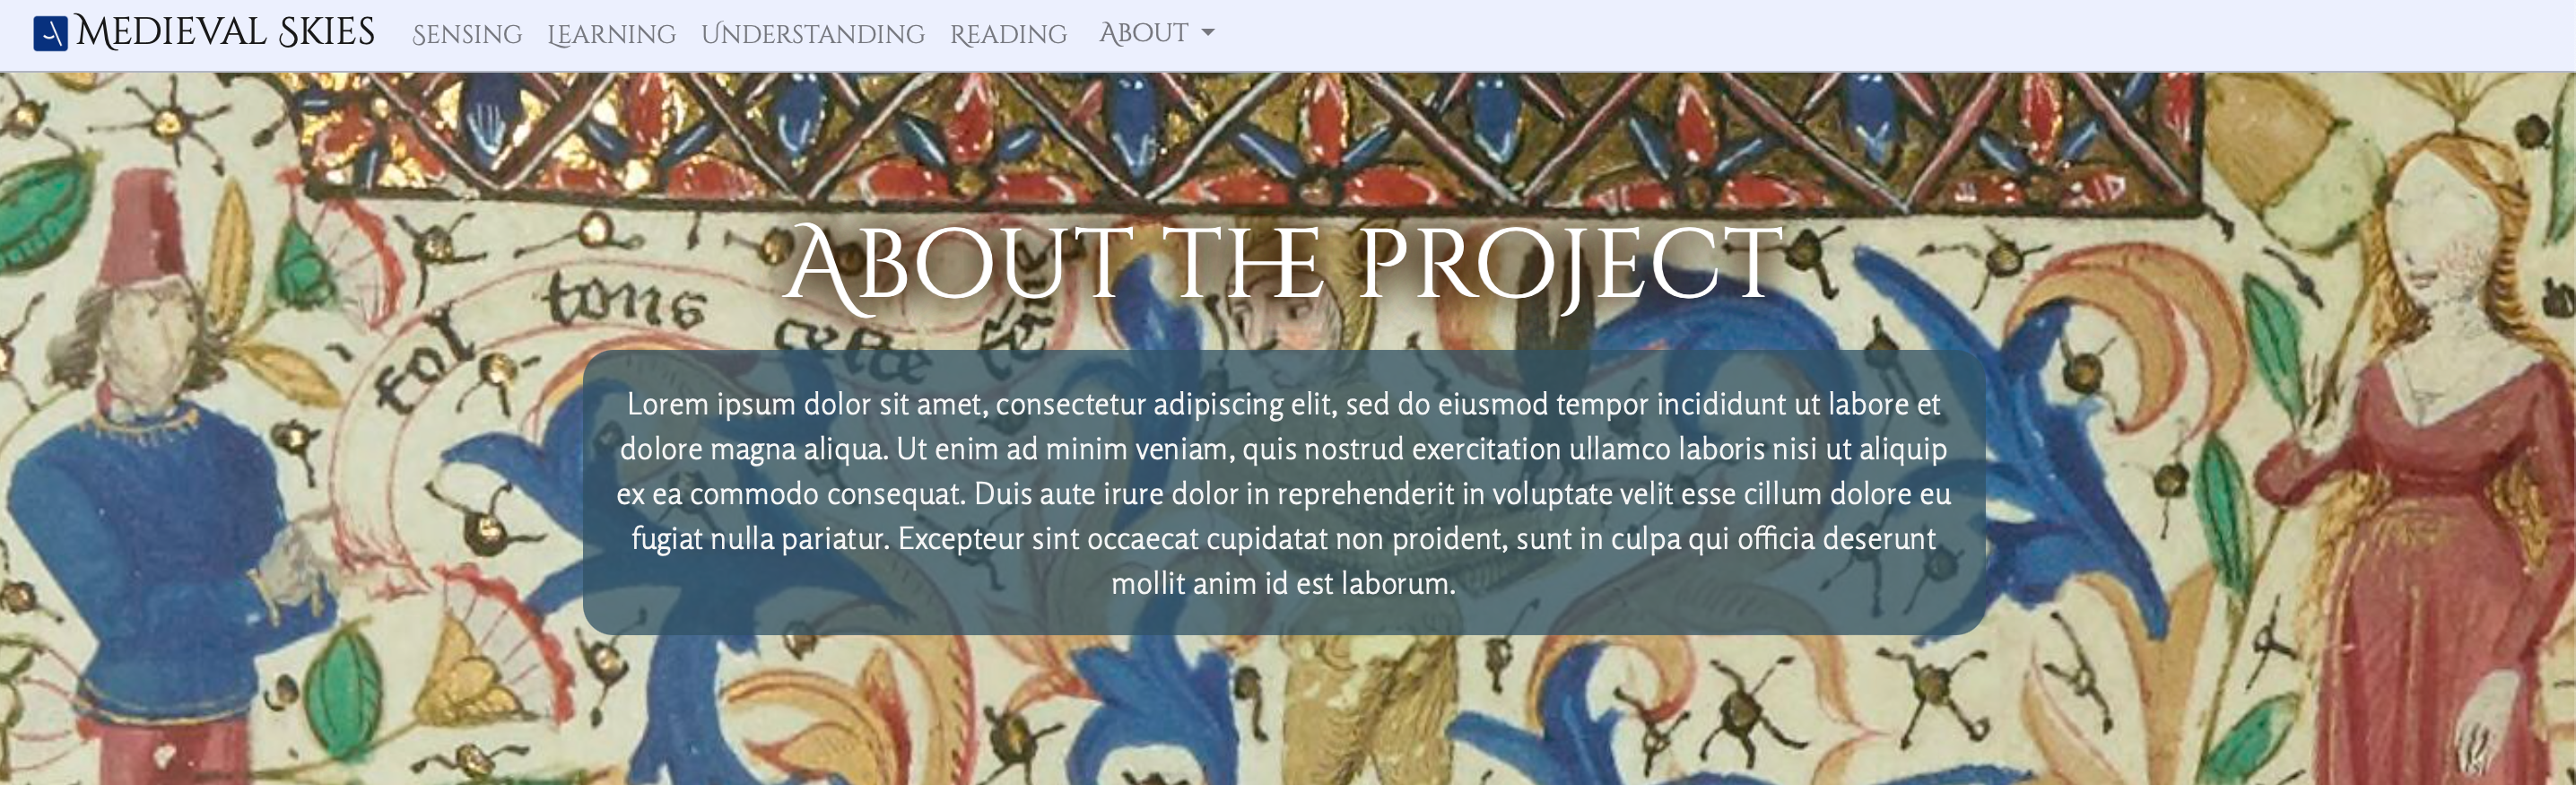
\includegraphics[width=\textwidth]{images/partie3/website/expo-about.png}
    \end{subfigure}
    \begin{subfigure}[h]{0.5\textwidth}
        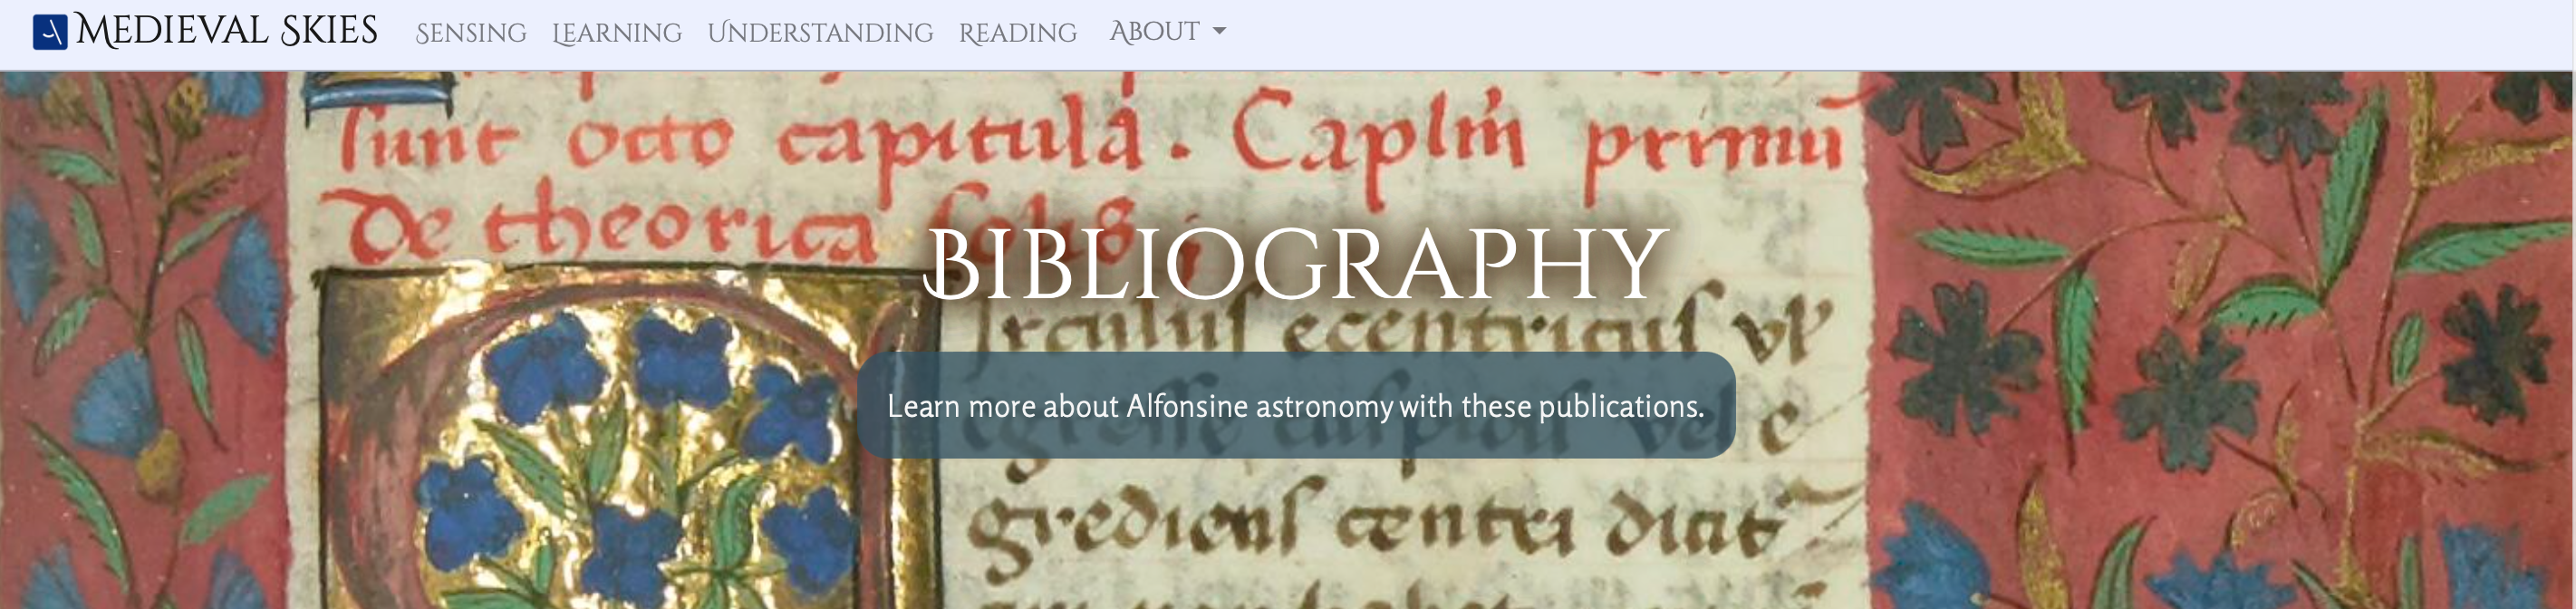
\includegraphics[width=\textwidth]{images/partie3/website/expo-bibliography.png}
    \end{subfigure}
    \begin{subfigure}[h]{0.5\textwidth}
        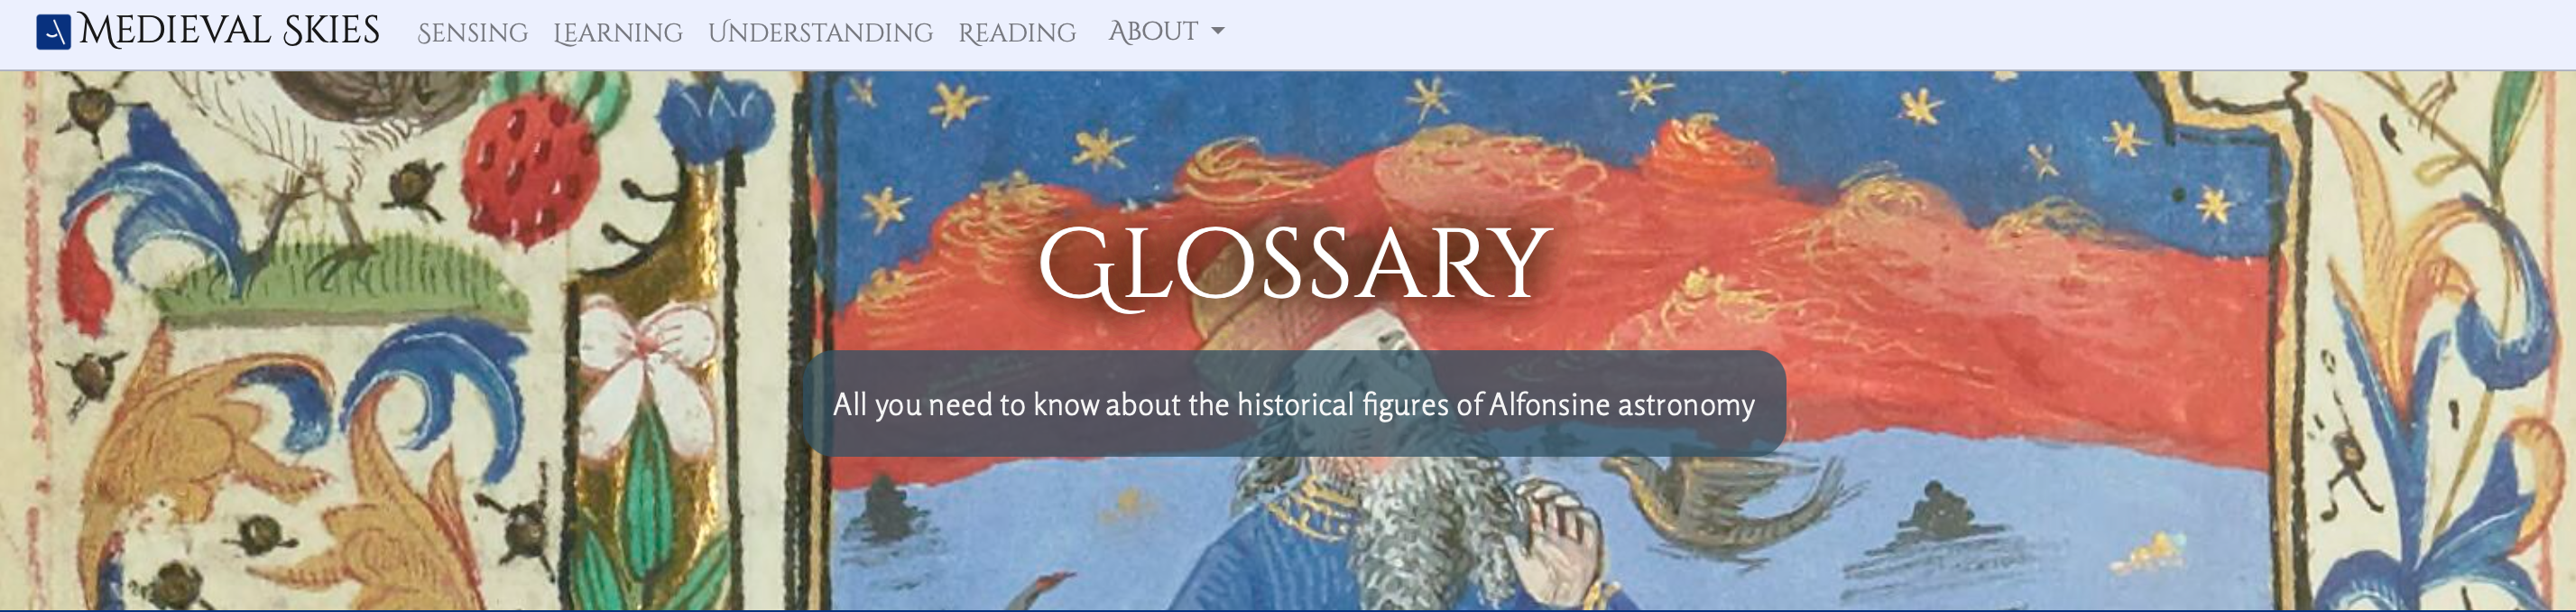
\includegraphics[width=\textwidth]{images/partie3/website/expo-glossary.png}
    \end{subfigure}
    \caption{Pages \textit{About this project}, \textit{Bibliography} et \textit{Glossary} du site \textit{Medieval skies under(book)cover}}
    \end{figure}

    \subsection{Ajouter, modifier ou supprimer des éléments}
    
    \subsubsection{Ajouter, modifier ou supprimer une page}
    On s'intéresse ici aux pages qui ne sont pas des thèmes ou des parcours, elles sont actuellement au nombre de quatre : \textit{Home}, \textit{About this project}, \textit{Bibliography} et \textit{Glossary}. Il sera possible d'en ajouter d'autres comme une page donnant accès à une carte précisant les lieux de conservation des manuscrits et ceux de production des textes qu'ils renferment, parmi les autres pages à créer on peut aussi évoquer la section jeu. L'ajout se fait en suivant quelques étapes : la première est de se rendre dans le fichier \texttt{routes.py} et d'y définir la fonction qui permettra d'inclure cette nouvelle page l'exposition. Prenons l'exemple de la page \textit{About}: 
    
    \begin{minted}{python}
    @app.route("/about", methods=["GET"])
    def about():
    return render_template(
        "pages/about.html",
         title="About",
         theme=main_pages["about"],
    )
    \end{minted}

    L'étape suivante consiste en une modification du fichier \texttt{paths.py}, il faut se rendre dans le dictionnaire appelé \texttt{main\_pages} où le nom de la page est utilisé comme clé et les informations relatives à la pages les valeurs.

    \begin{minted}{python}
    "about": {
    "url": "/about",
    "img": "static/img/cards/main-pages/about.jpg",
    "iiif": "https://gallica.bnf.fr/iiif/ark:/12148/btv1b100202503/f331/141,2291,1533,672/full/0/native.jpg",
    "header": "About this project",
    },
    \end{minted}

    Voici à quoi correspondent les différents éléments :
    \begin{itemize}
    \item \texttt{url} : \acrshort{url} de la page en cours de création
    \item \texttt{img} : image utilisée pour l'arrière plan du parallax
    \item \texttt{iiif} : lien vers l'image utilisée pour l'arrière plan du parallax au format \acrshort{iiif}
    \item \texttt{header} : titre de la page
    \end{itemize} 

    Si nécessaire, il faut ensuite ajouyter la page à la \textit{navbar} dans le fichier \texttt{navbar.html} où un élément \texttt{<a class="dropdown-item">}.

    \begin{minted}{html}
    <li class="dropdown">
        <button class="btn btn-secondary dropdown-toggle" type="button" id="dropdownMenuButton" data-toggle="dropdown" aria-haspopup="true" aria-expanded="false">About
        </button>
        <div class="dropdown-menu" aria-labelledby="dropdownMenuButton">
         <a class="dropdown-item" href="{{url_for('about')}}">About the project</a>
            <a class="dropdown-item" href="{{url_for('bibliography')}}">Bibliography</a>
            <a class="dropdown-item" href="{{url_for('glossary')}}">Glossary</a>
        </div>
    </li>
    \end{minted}

    Effectuer des modifications se fait de la même manière dans les différents fichiers mentionnés en laissant simplement de côté les étapes de création. 

    \subsubsection{Ajouter, modifier ou supprimer un thème ou un parcours}
    De façon assez analogue à l'ajout des autres pages, il faut d'abord définir une fonction dans le fichier \texttt{routes.py}. 
    
    Pour les thèmes, en prenant l'exemple du thème \textit{Sensing}\footnote{Avant d'avoir des noms définitifs pour les noms des thèmes, \textit{heritage}, \textit{historical}, \textit{scientific} et \textit{manuscripts} désignaient respectivement les thèmes \textit{Sensing}, \textit{Learning}, \textit{Understanding} et \textit{Reading}, c'est pour cette raison qu'ils sont ainsi désignés dans le code } : 
    \begin{minted}{python}
        @app.route("/heritage", methods=["GET"])
         def heritage():
            return theme_page("Heritage", "heritage", heritage_trails)
    \end{minted}
    
    Pour les parcours, avec l'exemple du parcours \textit{Seeing the manuscript} : 
    \begin{minted}{python}
        @app.route("/heritage/seeing", methods=["GET"])
        def seeing():
            return trail_page("Seeing the manuscript", "seeing", heritage_trails)
    \end{minted}
    
    Ensuite, le fichier \texttt{paths.py} doit à son tour être modifié. Pour ajouter un thème, il faut effectuer les modifications dans le dictionnaire \texttt{all\_themes}. Pour un parcours, il faut les effectuer dans le dictionnaire correspondant au thème dont fait partie ce parcours. 
    
    Pour les thèmes, en prenant l'exemple du thème \textit{Sensing} :
    \begin{minted}{python}
    "heritage": {
        "url": "/heritage",
        "img": "static/img/cards/main-pages/heritage.jpg",
        "iiif": "https://gallica.bnf.fr/iiif/ark:/12148/btv1b100202503/f459/133,1157,1262,490/full/0/native.jpg",
        "header": "Heritage trails",
        "category": "Focus on the material dimension of the manuscripts (the manuscript that we touch), on the visual aspects (the manuscript that we see) and the intellectual aspects (the manuscript that we read).",
        "color": "var(--heritage-color)",
        "parallax": "var(--parallax-heritage)",
    },
    \end{minted}
    
    Pour les parcours, avec l'exemple du parcours \textit{Seeing the manuscript} : 
    
    \begin{minted}{python}
    "seeing": {
        "url": "/heritage/seeing",
        "img": "static/img/cards/heritage/seeing.jpg",
        "iiif": "https://gallica.bnf.fr/iiif/ark:/12148/btv1b100202503/f261/159,197,322,555/800,/0/native.jpg",
        "category": "Discover",
        "header": "Seeing the manuscript",
        "color": "var(--heritage-color)",
        "exhibit": "https://www.exhibit.so/exhibits/3Ka2M3S7md6pdLZBy22C?embedded=true",
    },
    \end{minted}
    
    Les informations qui constituent les valeurs de ces dictionnaires sont tout à fait similaires qu'il s'agisse des thèmes ou des parcours : 
    \begin{itemize}
    \item \texttt{url} : \acrshort{url} de la page en cours de création
    \item \texttt{img} : image utilisée pour l'arrière plan du parallax ; l'image doit être enregistrée plutôt qu'utiliser celle au format \acrshort{iiif} car sinon le temps de chargement est bien trop important.
    \item \texttt{iiif} : lien vers l'image utilisée pour l'arrière plan du parallax au format \acrshort{iiif}
    \item \texttt{header} : titre du thème ou du parcours
    \item \texttt{category} : pour les thèmes, desciption de celui-ci ; pour les parcours, \og{}Discover\fg{} qui apparait sur les cartes
    \item \text{color} : couleur de fond de la page pour les thèmes, de fond de la section réservée au carrousel pour les parcours (la couleur utilisée est la même pour le thème et les parcours qui en font partie)
    \item \texttt{parallax} : couleur de fond du texte de description dans la section parallaax
    \item pour les parcours seulement, \texttt{exhibit} : lien vers l'\textit{exhibit} créé pour ce parcours
    \end{itemize} 
    
    Les couleurs sont définies comme variables dans le fichier \texttt{style.css}. Les thèmes doivent aussi être ajoutés à la barre de navigation afin d'être accessibles depuis l'intégralité des pages du site web. Le procédé est le même que pour les autres pages, à la différence que les thèmes ne sont pas ajoutés au menu déroulant. 
    
    \begin{minted}{html}
    <li class="nav-item">
        <a class="nav-link" href="{{url_for('heritage')}}" 
        title="Material aspect of the manuscript">Heritage</a>
    </li>
    \end{minted}
    
    Là encore, pour effectuer des modifications ou des suppression, ce sont les mêmes fichiers qui doit être retravaillés. 
    
    \subsubsection{Ajouter, modifier ou supprimer une entrée au glossaire}
    Dans ce cas, il n'y a pas de page à créer car la structure de la page \textit{Glossary} existe déjà, il s'agit simplement d'ajouter de nouvelles entrées ou de modifier celles qui sont déjà intégrées. Cela passe par le fichier \texttt{persons.py}. Dans le dictionnaire \textit{persons}, les informations liées à un personnage peuvent être ajoutées en valeurs tandis que son nom est la clé de ce couple clé/valeur :
    
    \begin{itemize}
        \item \texttt{name} : nom de l'astronome 
        \item \texttt{url} : \acrshort{url} de la page Wikipedia, si elle existe
        \item \texttt{biography} : éléments de biographie (à rédiger)
        \item \texttt{attention\_points} : folio(s) mentionnant le personnage et le lien de l'\textit{attention point} correspondant (il faut être vigilant à reporter le lien précis de l'\textit{attention point} et non pas celui qui renverrait le visiteur au début de l'\textit{exhibit}
        \item \texttt{id\_biblissima} : identifiant de l'astronome dans la base de données Biblissima, quand cette donnée est disponible
    \end{itemize}
    
    
    Illustrons cela avec la première entrée du glossaire : 
    \begin{minted}{python}
    "albumazar": {
        "name": "Abu Ma'shar",
        "url": "",
        "biography": "",
        "attention_points": {
            manuscripts_trails["bnf7281"]["header"]: {
                "f. 237v": "https://www.exhibit.so/exhibits/pByGoZQTs7Y0d5RA1EXk?screen=ywWveU59hwK7G4Aap3er"
            },
            manuscripts_trails["bnf7286c"]["header"]: {
                "f. 55r": "https://www.exhibit.so/exhibits/tPKyQQcpctVpM4tzsTnu?screen=qfI07VfoYKZX59dOJlEa"
            },
            manuscripts_trails["basel7"]["header"]: {
                "f. 82r": ""
            },
        },
        "id_bliblissima": "Q624",
    },
    \end{minted}
    
    Une fois les pages créées, il est donc aisé de modifier leur contenu. De plus quel que soit l'élément que l'on souhaite changer, les étapes à suivre sont très similaires ce qui rend la prise en main plutôt facile. 

	\section{Réalisation d’une exposition modulaire}
	Ce site est conçu grâce à une application flask. Flask est un module Python qui permet de développer des applications de manière plutôt simple. Au sein de cette application, des \textit{templates} sont utilisés pour différents éléments utilisés à plusieurs endroits. Procéder de la sorte rend la réutilisation de ces éléments simple quand elle est nécessaire. Lors de la conception de cette exposition, l'idée été de concevoir quelque chose qui puisse être modulé aisément selon les besoins, notamment pour être en mesure d'ajouter un manuscrit ou un parcours le cas échéant. Ainsi des \textit{templates} existent pour la création des pages de thèmes et de parcours mais aussi pour ajouter des carrousels, des \textit{cards} ou des \textit{exhibits}, par exemple. 
	
    \subsection{Création de fonctions}
    La création de contenu modulaire en python passe par la définition de fonctions. Pour les pages qui font appel à des \textit{templates}, ces fonctions prennent des paramètres plus nombreux comme le montre l'exemple de la fonction créée pour les pages des principaux thèmes \footnote{Les autres fonctions créées en suivant le même principe peuvent être consultées en annexe \ref{Fonctions}, à la page \pageref{Fonctions}.} :  
    \begin{minted}{python}
    def theme_page(title, theme_name, theme_trails, themes=all_themes):
        trails = list(theme_trails.values()) 
        #permet de placer les cards dans un ordre aléatoire:
        random.shuffle(trails) 
        return render_template(
            "pages/theme.html",
            title=title,
            id=theme_name,
            theme=themes[theme_name],
            cards=trails,
            #permet de retirer le thème où l'on se trouve du carrousel:
            carousel_items=remove_item(themes, theme_name),
        )
    \end{minted}
    
    Ces fonctions peuvent alors être appelées au gré des besoins et des évolutions du contenu de l'exposition. C'est le cas pour chacune des pages des principaux thèmes, ici avec l'exemple du thème \textit{Learning} :
    
    \begin{minted}{python}
    def historical():
        return theme_page("Historical", "historical", historical_trails)
    \end{minted}
    
    Si un thème vient à être ajouté, il suffira donc de créer la route dans le fichier \texttt{route.py}, comme expliqué dans la partie précédente, et de faire appel à la fonction \texttt{theme\_page}. De façon analogue, les pages des parcours font, quant à elles, appel à la fontion \texttt{trail\_page}. Là encore, pour ajouter un parcours les seules exigences sont la création de la route et l'appel de la fonction. 
    
	\subsection{Création de \textit{templates}}
	Une fois les fonctions en place, il est nécessaire de fournir le code \acrshort{html} qui permettra d'afficher le contenu sur le navigateur des visiteurs. Là encore, plutôt que de créer un fichier \acrshort{html} pour chacune des pages de l'exposition, le contenu commun a été mutualisé, sur les conseils de Ségolène Albouy. Cela constitue une bonne pratique qui permet de rendre le code plus clair et plus propre et qui facilite également sa modification et sa prise en main par des tiers. Ainsi des \textit{templates} ont, une fois de plus, été créés pour les pages de thèmes et de parcours. \footnote{L'ensemble des \textit{templates} utilisés pour le développement de l'interface de l'exposition fait partie des livrables techniques}.
	
	Au sein de ces \textit{templates} principaux, d'autres, plus petits car relatifs à un élément de la page plutôt qu'à son architecture complète, sont appelés et concernent notamment des éléments \acrshort{css} tels que les carrousels présents en bas de ces pages pour accéder aux autres thèmes ou autres parcours, les \textit{cards} qui permettent aux visiteurs de choisir un parcours au sein d'un thème ou encore les parallax qui sont la section supérieure de l'ensemble des pages du site où l'on trouve le titre et une description sommaire du contenu de la page. 
	De même pour les parcours, l'insertion des \textit{exhbits} se fait par le biais d'un \textit{template}. Pour la création du glossaire, c'est encore une fois ce même système qui est mis en place. 
	
	Les éléments à afficher sur les pages présentant un contenu similaire sont renseignés dans des dictionnaires regroupés dans le fichier \texttt{utils}. Le fait d'avoir des dictionnaires permet d'utiliser des boucles pour que le contenu associé à chacun des éléments soit affiché correctement mais en ayant seulement quelques lignes de code plutôt qu'un code très long avec un fichier \acrshort{html} pour chaque page qui contiendrait des répétitions nombreuses des mêmes morceaux de code. Ainsi, un \textit{template} utilisant une boucle indiquant ce qui doit être affiché pour chaque parcours dans le dictionnaire relatif à un thème est préférable à la répétition quatre fois, si il y a quatre parcours, d'un code identique dans sa structure mais où le contenu est spécifique à chaque parcours. Procéder ainsi permet enfin d'éviter, ou au moins de réduire, les erreurs qui se glisseraient inévitablement dans un code construit de la sorte. 
	
	\chapter{Mise en valeur des données}
	Dans cet ultime chapitre, on s'efforce de porter un regard critique sur la mise en valeur des données de la recherche grâce à l'exposition \textit{Medieval skies under(book)cover} en évoquant des questionnements sur le rendu esthétique du site web avant de dire quelques mots du futur de l'exposition.
	\section{Une interface au service des visiteurs}
	\subsection{Création d'une exposition \textit{responsive}}
	Un site web \textit{responsive} est un site qui peut s'accommoder à toutes les tailles et résolutions d'écran. Il s'agit d'adapter l'affichage des éléments d'une pages aux différents supports que les visiteurs peuvent utiliser : ordinateurs, tablettes et \textit{smartphones}. Le contenu n'est donc pas propre à chaque support mais il est adapté à chacun d'entre eux.  À l'heure où l'utilisation des \textit{smartphones} est omniprésente, il semble important de pouvoir proposer un contenu auquel les visiteurs pourront avoir accès depuis leur \textit{smartphones}. En effet, ne pas considérer cette possibilité serait exclure dès le départ une partie du public ciblé qui cherche a avoir accès à un contenu instantané. 
	
	À l'échelle globale du site web, l'affichage du contenu des pages est harmonisé pour les différentes tailles d'écrans dans le fichier \texttt{style.css} : 
	\begin{minted}{css}
	@media screen and (min-width: 900px) {
        .page-title {
            font-size: 4rem;
        }
        .main-content {
         max-width: 40vw;
        }
        .main-item {
            width: 55vw;
        }
        .div-main-content {
            height: 40vw;
        }
    }

    @media screen and (min-width: 500px) and (max-width: 900px) {
        .page-title {
            font-size: 5rem;
        }
        .main-content {
            max-width: 80vw;
        }
        .main-item {
            width: 85vw;
        }
        .div-main-content {
            height: 81vw;
        }
        #parallax-title {
            font-size: xxx-large;
        }
    }

    @media screen and (max-width: 500px) {
        .page-title {
            font-size: 10vw;
        }
        .main-content {
            max-width: 90vw;
        }
        .main-item {
            width: 90vw;
        }
        .div-main-content {
            height: 92vw;
        }
        .add-lg {
            display: none;
        }
        #parallax-title {
            font-size: xx-large;
        }
    }
	 \end{minted}
	 
	 Il est ainsi possible de paramétrer l'affichage des titres et du contenu selon selon la taille des écrans, pour avoir un résultat le plus adapté possible, on définit trois tailles d'écran qui correspondent plus ou moins aux ordinateurs, tablettes et \textit{smartphones}.
	 Néanmoins, pour des écrans de petite taille, il n'est pas exclu de faire le choix de pas afficher certains éléments : c'est le cas sur la page \textit{Glossary} pour les \textit{smartphones} où le listing des folios n'apparaît pas pour privilégier le contenu biographique\footnote{Une comparaison des trois écrans est disponible en annexe \ref{ResponsiveScreen}, à la page \pageref{ResponsiveScreen}.}. De la même manière, sur les pages des thèmes, le nombre de cartes affichées sur une même ligne varie selon la taille de l'écran. Ces paramètres sont à régler dans le \acrshort{css} du fichier à l'intérieur de la balise \texttt{<style>}.

    Néanmoins, malgré ces efforts il faut noter que tous les contenus ne sont pas parfaitement adaptés à tous les types d'écran. Par exemple, sur la page d'accueil, un manuscrit cliquable a été ajouté en utilisant une image vectorielle. Malgré des difficultés de calibrage du \acrshort{svg} pour que les zones cliquables correspondent aux bonnes coordonnées de l'image quelle que soit la taille de l'écran, ce problème a pu être résolu. Toutefois, demeure le fait que sur un écran tactile le visiteur n'a pas d'indication sur cette fonctionnalité alors que sur un écran non tactile, au survol de la souris la zone cliquable est grisée : cela indique au visiteur que c'est une zone cliquable.  

    \subsection{Réflexion sur l'esthétique du site web}
    Si le principal élément de mise en valeur des manuscrits vient des \textit{exhibits}, cela n'exclue pas le reste du site web d'y contribuer. En effet, l'objectif est donc de permettre aux visiteurs d'avoir une progression fluide jusqu'à la navigation au sein d'un \textit{exhibit} et donc d'un parcours. 
    Un code couleur très simple aide les visiteurs à se repérer dans leur navigation : la couleur principale utilisée pour un thème est également présente sur les pages des parcours issus de celui-ci. Cela aide les internautes à déambuler dans cette exposition en sachant rapidement que les pages qu'ils consultent sont ou non associées. Pour être bien sûre que les couleurs utilisées soient identiques quand elles doivent l'être des variables ont été créées afin de réutiliser très commodément ces couleurs lors de l'implémentation du \acrshort{css} des différents éléments des pages web. 
    
    \begin{minted}{css}
    --heritage-color: #518cb0;
    --parallax-heritage: rgba(55, 78, 113, 0.75);
    --historical-color: #757055;
    --parallax-historical: rgba(48, 52, 41, 0.75);
    --scientific-color: #dcccb5;
    --parallax-scientific: rgba(62, 51, 42, 0.75);
    --manuscripts-color: #862b28;
    --parallax-manuscripts: rgba(99, 26, 21, 0.75);
    \end{minted}
    
    La couleur étant un élément de cohérence, les couleurs choisies pour chacun des thèmes renvoient à celles du manuscrit \acrshort{svg} de la page d'accueil : dès le départ, le visiteur peut donc associer une couleur à une thématique. De plus, lors de l'ajout des \textit{shortcuts}, on peut envisager l'utilisation de ces mêmes couleurs pour signaler au vsiteur qu'il est conduit vers une autre thématique.
    
    Par ailleurs, pour les pages considérées comme annexes, dans le sens où elles ne concernent pas les parcours d'exposition, la couleur qui a été choisie est la nuance de bleu qui est utilisée sur d'autres site web du projet \acrshort{alfa} afin de, là aussi, créer de la cohérence à l'échelle globale du projet. \\
    
    Enfin, pour fluidifier la progression au sein de l'exposition, des titres clairs ont du être choisis pour les thèmes majeurs mais également pour l'exposition elle-même. Autre preuve du dialogue entre les différentes personnes prenant part au projet, tous ceux qui le souhaitaient ont pu proposer des titres qui ont ensuite été soumis à un vote parmi les membres de l'équipe. Ces titres devaient satisfaire les besoins scientifiques de clarté pour aiguiller les visiteurs tout en se pliant à des contraintes techniques, voire esthétiques, d'intégration au site web. Ainsi, le titre devait pouvoir avoir une version courte pour la barre de navigation. De même les titres des thèmes devant également être ajoutés à la \textit{navbar}, ils ne devaient pas non plus être trop longs, idéalement un seul mot.

	\section{Futur de cette exposition virtuelle}
	Si l'objectif d'avoir une interface d'exposition est atteint, cela ne signifie pas que ce projet de \textit{digital exhibition} est pour autant achevé. Premièrement, un certain nombre d'\textit{attention points} est encore à compléter. Ensuite doivent être envisagés l'ajout des parcours raccourcis, avec la sélection des \textit{attention points} qui en feront parti, et le choix des \textit{must see}. Le cas du manuscrit de l'Université de Bâle, disponible uniquement sous microfilms, doit aussi être statué car, en l'état, il ne peut être inclus à une exposition virtuelle. Les pages annexes devront aussi être complétées afin d'offrir aux internautes l'intégralité des ressources utiles à leur compréhension de l'astronomie alphonsine. Tout cela correspond à des points connus de l'équipe et leur réalisation est déjà prévue. 
	
	D'autre part, on peut également penser à des idées de plus grande envergure pour compléter cette première version de l'exposition. Un premier projet dont il est déjà question est de proposer aux internautes de visiter l'exposition \textit{Medieval skies} dans une autre langue que l'anglais. Le caractère international de l'équipe offre des possibilités pour le français, l'italien ou encore l'espagnol. Cela signifierait aussi une expansion de l'audience. En effet, si nombreuses sont les personnes qui peuvent comprendre l'anglais, avoir la possibilité de bénéficier de cette expérience dans sa langue maternelle serait une valeur ajoutée à l'exposition. De plus, le contenu de l'exposition a pu être évoqué comme possible complément d'un contenu pédagogique lié au programme scolaire et, là encore, la possibilité d'y accéder dans d'autres langues que l'anglais serait bienvenue. 
	
	Enfin, ce projet peut facilement être augmenté par l'ajout d'autres manuscrits ou d'autres parcours grâce à l'utilisation de \textit{templates}. Cette éventualité prendrait place au sein du projet \acrshort{alfa} mais ce n'est pas la seule possibilité. En effet, on peut aussi imaginer une vie en dehors de l'Observatoire de Paris, pour l'exposition peut-être mais pour son modèle plutôt. Ainsi, du fait de son architecture simple, facilement prise en main et aisément adaptable, \textit{Medieval skies under(book)cover} pourrait servir de modèle à une autre exposition qui serait construite de façon analogue avec des thèmes subdivisés en plusieurs parcours. Cela irait dans le sens des humanités numériques comme facteur de partage, de collaboration et de science ouverte. \\
	
	Cette ultime partie consacrée au développement effectif d'une interface permettant la mise en valeur du corpus alphonsin a permis de mettre en avant le dynamisme de la communauté \acrshort{iiif} et l'intérêt de ces images haute définition pour exposer de précieux manuscrits. Pour développer le site web, le choix a été fait d'une architecture simple et facilement modulable afin de rendre la réutilisation du code la plus simple posisble. Enfin, une réflexion a été portée sur la mise en valeur des données et les possibles axes d'amélioration pour le futur. 

